\documentclass[10pt,a4paper]{book}
\usepackage{cancel}

\def\scale{.455}
\NewDocumentCommand\Phiz{}{\Phi_{\bm{x}}}
\NewDocumentCommand\Phix{m}{\Phi_{\bm{x}_{#1}}}
\NewDocumentCommand\nKL{}{Kullback--Leibler}
\NewDocumentCommand\KKT{}{Karush--Kuhn--Tucker}
\NewDocumentCommand\dmd{}{\texttt{dmd}}
\NewDocumentCommand\xxd{}{\texttt{xxd}}
\NewDocumentCommand\huff{}{\texttt{huff}}

\book{Scalaで実装するパターン認識と機械学習}{Scala's Pattern Recognition {\&} Machine Learning}{3}{データマイニング,サポートベクターマシン}

\begin{document}
\maketitle
\tableofcontents

\chapter{回帰とクラス分類の基礎\label{chap:intro}}

機械学習とは、$\bm{y}=f(\bm{x})$に従うデータ集合$\seq{\bm{x}_n,\bm{y}_n}$に対し、関数$f$を推定するアルゴリズムの総称である。
\chapref{intro}では、機械学習の初歩的な事例として\textbf{線型回帰}と\textbf{最近傍法}を実装し、機械学習の感覚的理解を目指す。

\section{線型回帰\label{sect:intro.reg}}

機械学習の中でも、標本$\seq{\bm{x}_n,\bm{y}_n}$が入力$\bm{x}$に対する出力$\bm{y}$を明示的に指定する場合を\textbf{教師あり学習}と呼ぶ。
教師あり学習の中でも、出力すべき変数$\bm{y}$が連続値を取る場合を\textbf{回帰}と呼び、線型回帰はその初歩と言える。
線型回帰は、\eqref{reg.basic}に示す通り、従属変数$y$を自由変数$x_k$に加重$w_k$を掛けた和で説明するモデルである。
%
\begin{equation}
\label{eq:reg.basic}
y = f(\bm{x}) = w_0 + \sum_{k=1}^K w_k x_k
= \begin{pmatrix} w_0 \\ w_1 \\ \vdots \\ w_K\end{pmatrix} \cdot \begin{pmatrix} 1 \\ x_1 \\ \vdots \\ x_K\end{pmatrix}
= \trans{\bm{w}} \bm{x}.
\end{equation}

また、何らかの非線型な写像$\phi_k(\bm{x})$の線型結合で回帰を行う\eqref{reg.basis}のモデルを\textbf{線型基底関数モデル}と呼ぶ。
%
\begin{equation}
\label{eq:reg.basis}
y = f(\bm{x}) = \sum_{k=0}^K w_k \phi_k(\bm{x}) = \trans{\bm{w}}\bm{\phi}(\bm{x}).
\end{equation}

\figref{reg.cubic}は$y\!\sim\!\Nd{y|x^3\!-\!3x,2500}$に従う$\seq{x_n,y_n}$に$\phi_k(x)\!=\!x^k$の線型基底関数モデルを適用した例である。

\begin{figure}[h]
\centering
\subfloat[]{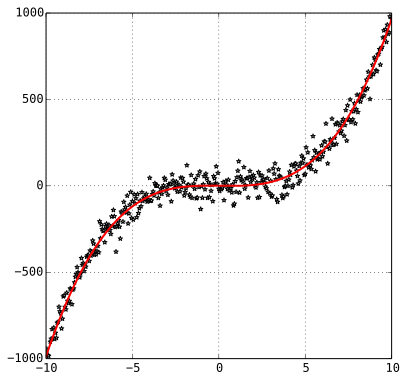
\includegraphics[width=.5\linewidth]{images/reg.plot1.eps}}
\subfloat[]{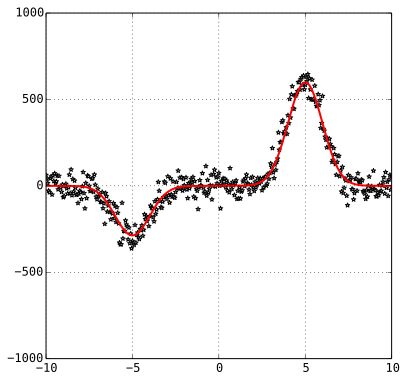
\includegraphics[width=.5\linewidth]{images/reg.plot2.eps}}
\caption{linear basis function model.\label{fig:reg.cubic}}
\end{figure}

線型基底関数モデルでは、他にも$\phi_k(x)\!=\!\Nd{x|\mu_k,\sigma_k^2}$を採用すれば、$\mu_k$近傍の局所的な曲線を表現できる。
%
\begin{equation}
y = f(\bm{x}) = \left\{
\begin{aligned}
&\sum_{k=0}^K w_k x^k&
&\where \phi_k(x)=x^k,\\
&\sum_{k=0}^K \frac{w_k}{\sqrt{2\pi\sigma_k^2}}\exp\left\{-\frac{(x-\mu_k)^2}{2\sigma_k^2}\right\}&
&\where \phi_k(x)=\Nd{x|\mu_k,\sigma_k^2}.
\end{aligned}
\right.
\end{equation}

実際の観測にはノイズ$\varepsilon_n$が重畳する。ノイズは釣鐘型に分布するので、正規分布を仮定して\eqref{reg.noise}を得る。
%
\begin{equation}
\label{eq:reg.noise}
y = f(\bm{x}) + \varepsilon \sim p(y|\bm{x},\bm{w},\beta) = \Nd{y|f(\bm{x}),\beta^{-1}}.
\end{equation}

なお、$\beta$は分散の逆数で、ノイズの\textbf{精度}である。観測された標本$\seq{\bm{x}_n,y_n}$の出現確率は、\eqref{reg.like}で求まる。
%
\begin{equation}
\label{eq:reg.like}
p(\seq{y_n}|\seq{\bm{x}_n},\bm{w},\beta) = \prod_{n=1}^N \Nd{y_n|\trans{\bm{w}}\bm{\phi}(\bm{x}_n), \beta^{-1}}.
\end{equation}

\eqref{reg.like}を\textbf{尤度}と呼ぶ。尤度は、与えられた訓練データを良く表現する\textbf{母数}としての加重$\bm{w}$の妥当性を示す。
線型回帰の学習は、尤度の最大化を目指す。今回は、計算の容易性から、\eqref{reg.like.log}の対数尤度を最大化する。
%
\begin{equation}
\label{eq:reg.like.log}
\log p(\seq{y_n}|\seq{\bm{x}_n},\bm{w},\beta)
= \frac{N}{2}\log\beta - \frac{N}{2}\log2\pi - \frac{\beta}{2}\sum_{n=1}^N\{y_n-\trans{\bm{w}}\bm{\phi}(\bm{x}_n)\}^2.
\end{equation}

\eqref{reg.like.log}から定数項を取り除き、加重$\bm{w}$に依存する項を取り出すと、\eqref{reg.error}の2乗誤差関数$E(\bm{w})$を得る。
\eqref{reg.error}の最小化は、\textbf{最小二乗法}とも呼ばれる。さて、誤差$E(\bm{w})$を最小化する具体的な方法を検討しよう。
%
\begin{equation}
\label{eq:reg.error}
E(\bm{w}) = \frac{1}{2} \sum_{n=1}^N \left\{y_n - \sum_{k=0}^K w_k \phi_k(\bm{x}_n)\right\}^2.
\end{equation}

誤差$E(\bm{w})$は\textbf{連続関数}なので、勾配$\nabla E(\bm{w})$が0の点で最小になる。ここで、\eqref{reg.grad}の\textbf{勾配法}を導入する。
勾配法とは、加重$\bm{w}$を極値に向けて動かす操作を繰り返し、最終的に$\nabla E(\bm{w})=0$で収束させる手法である。
%
\begin{equation}
\label{eq:reg.grad}
\bm{w}' = \bm{w} - \eta \nabla E(\bm{w}) = \bm{w} + \eta \sum_{n=1}^N \{y_n - \trans{\bm{w}} \bm{\phi}(\bm{x}_n)\} \bm{\phi}(\bm{x}_n).
\end{equation}

係数$\eta$は\textbf{学習率}と呼ばれ、加重$\bm{w}$の発散を防止するため、$\eta\nabla E(\bm{w})\ll{}\bm{w}$となるように調整する必要がある。
勾配法による線型回帰を\texttt{Regression}クラスに実装する。引数\texttt{e}は学習率$\eta$で、\texttt{XY}は標本$\seq{x_n,y_n}$を表す。

\begin{Verbatim}{Scala}
class Regression(e: Double, XY: Seq[(Double, Double)], p: Seq[Double=>Double]) {
	val w = Array.fill[Double](p.size)(0)
\end{Verbatim}

配列\texttt{p}は、写像$\phi_k(x)$を格納する長さ$K$の列$\seq{\phi_k}$である。下記の\texttt{apply}メソッドは、\eqref{reg.basis}を計算する。

\begin{Verbatim}{Scala}
	def apply(x: Double) = w.zip(p.map(_(x))).map{case (w,x)=>w*x}.sum
\end{Verbatim}

最後に、\eqref{reg.grad}による加重$\bm{w}$の更新を実装する。反復回数を固定せずに、収束判定を行うと実用的である。

\begin{Verbatim}{Scala}
	for(n<-1 to 1000; (x,y) <- XY; k<-0 until p.size) w(k) += e * (y-this(x)) * p(k)(x)
}
\end{Verbatim}

完成した\texttt{Regression}クラスに$y=x^3+\varepsilon$の標本を与えて、基底$\seq{x^3,x^2,x,1}$で線型回帰を行う例を示す。

\begin{Verbatim}{Scala}
val pts = -10.to(10).map(x=>(x.toDouble, math.pow(x,3) + util.Random.nextGaussian))
val reg = new Regression(0.000001, pts, 0.to(3).map(k=>(x: Double)=>math.pow(x,k)))
\end{Verbatim}

\chapref{nn}で学ぶ\textbf{ニューラルネットワーク}は、活性化関数を追加した線型基底関数モデルと本質的に等価である。

\section{最近傍法\label{sect:intro.knn}}

教師あり学習の中でも、従属変数$\bm{y}$が離散値を取る場合を\textbf{クラス分類}と呼び、最近傍法はその初歩と言える。
\subfigref{knn}{model}に示す最近傍法は、未知の点を分類する際に近傍の$k$点を参考にする。$k$の決め方が重要である。

\begin{figure}[h]
\centering
\subfloat[$k$ nearest neighbor diameters.\label{fig:knn:model}]{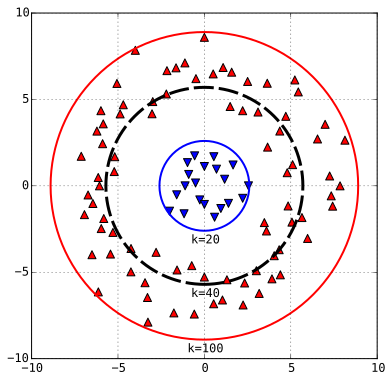
\includegraphics[width=.5\linewidth]{images/knn.model.eps}}
\subfloat[$k\!=\!10$ region segmentation.\label{fig:knn:judge}]{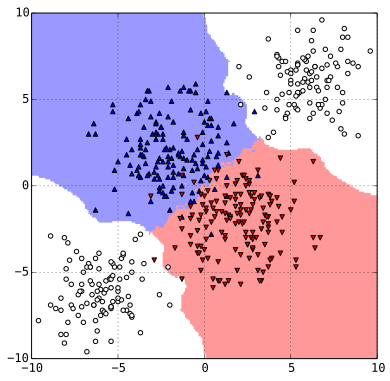
\includegraphics[width=.5\linewidth]{images/knn.judge.eps}}
\caption{$k$ nearest neighbor model.\label{fig:knn}}
\end{figure}

最近傍法は\textbf{遅延学習}とも呼ばれ、事前の学習処理が不要で、分類時に初めて標本を参照する点が特徴である。
下記の\texttt{KNN}クラスは、未分類の点と訓練データの各点との距離を計算し、最近傍の$k$個の点で多数決を行う。

\begin{Verbatim}{Scala}
class KNN[D,T](k: Int, data: Seq[(D,T)], d: (D,D)=>Double) {
\end{Verbatim}

引数\texttt{d}には距離関数$d$を指定する。例えば、\textbf{平方ユークリッド距離}を使うには、下記の\texttt{quad}関数を与える。

\begin{Verbatim}{Scala}
def quad(a: Seq[Double], b: Seq[Double]) = (a, b).zipped.map(_-_).map(x => x * x).sum
\end{Verbatim}

距離関数$d$の決め方は重要な課題である。典型的には平方ユークリッド距離や\textbf{マンハッタン距離}を採用する。
厳密には、\eqref{knn.dist}の\textbf{距離の公理}を満たす必要があるが、距離の比較ができれば、厳密な定義は不要である。
%
\begin{equation}
\label{eq:knn.dist}
\left\{
\begin{aligned}
d(\bm{x}, \bm{y}) &\geq 0, \\
\bm{x} = \bm{y} &\Leftrightarrow d(\bm{x}, \bm{y}) = 0, \\
d(\bm{x}, \bm{y}) &= d(\bm{y}, \bm{x}), \\
d(\bm{x}, \bm{y}) &\leq d(\bm{x}, \bm{z}) + d(\bm{z}, \bm{y}).
\end{aligned}
\right.
\end{equation}

下記の\texttt{apply}メソッドは、座標$\bm{x}$近傍の$k$点を引数\texttt{data}で与えた標本$\seq{\bm{x}_n,y_n}$から探し、多数決を採る。

\begin{Verbatim}{Scala}
	def apply(x: D) = data.sortBy(s=>d(x,s._1)).take(k).groupBy(_._2).maxBy(_._2.size)._1
}
\end{Verbatim}

\subfigref{knn}{judge}は、混合正規分布に従う標本を\texttt{KNN}クラスで学習して、変数$\bm{x}$の空間を塗り分けた結果である。
実用的には、距離計算の計算量を抑えるため、R木などの\textbf{空間データベース}で探索空間を局限すべきである。

\chapter{決定木の学習と汎化性能\label{chap:dec}}

\eqref{dec.swim}は、気象条件$\bm{x}$に対して質問と条件分岐を繰り返し、海水浴の是非$y$を判断する\textbf{決定木}の例である。
%
\begin{equation}
\label{eq:dec.swim}
y \approx f(\bm{x}) = \begin{cases}
0 & \text{if $\mathrm{wavy}(\bm{x}) = 1$} \\
\text{otherwise}
\left\{
\begin{aligned}
& 0 && \text{if $\mathrm{rain}(\bm{x}) = 1$} \\
& 1 && \text{if $\mathrm{rain}(\bm{x}) = 0$} \\
\end{aligned}
\right\}
& \text{if $\mathrm{wavy}(\bm{x}) = 0$} \\
\end{cases}
\end{equation}

理想的な決定木は、簡潔明瞭である。故に、決定木の学習は標本$\seq{\bm{x}_n}$に対する質問回数の最小化を目指す。
質問回数の最小化は、第\ref{sect:dec.info}に述べる\textbf{情報量の加法性}を勘案すれば、質問の\textbf{情報利得}の最大化と同義である。

\section{情報利得の最大化\label{sect:dec.info}}

ある確率分布に従う記号列$\seq{y_n}$を出力する装置を\textbf{情報源}と呼び、特定の情報$y$の価値$I(y)$を\textbf{情報量}と呼ぶ。
真に価値ある情報は、稀有な筈である。試みに、情報量$I(y)$を記号$y$の出現確率$P(y)$の反比例で定義する。
%
\begin{equation}
\label{eq:dec.info.bad}
I(y) = \frac{1}{P(y)}.
\end{equation}
%
\eqref{dec.info.bad}の定義は自然に思えるが、記号列$\seq{y_n}$の情報量$I(\seq{y_n})$を計算すると、\eqref{dec.info.seq}の違和感に気付く。
%
\begin{equation}
\label{eq:dec.info.seq}
I(\seq{y_n}) = \prod_{n=1}^N \frac{1}{P(y_n)} = \prod_{n=1}^N I(y_n).
\end{equation}
%
情報量が情報の価値を表す量であるなら、情報量$I(\seq{y_n})$は、情報量$\seq{I(y_n)}$の和になって然るべきである。
この直観を情報量の加法性と呼ぶ。そこで、対数関数を利用して、情報量$I(y)$の定義を\eqref{dec.info}で修正する。
%
\begin{equation}
\label{eq:dec.info}
I(y) = \log_2 \frac{1}{P(y)} = - \log_2 P(y) \geq 0.
\end{equation}
%
また、情報源$Y$に対し、情報量$I(y)$の期待値$H(Y)$を定義する。期待値$H(Y)$は\textbf{エントロピー}と呼ばれる。
%
\begin{equation}
\label{eq:dec.ent}
H(Y) = \sum_{y \in Y} P(y) I(y) = - \sum_{y \in Y} P(y) \log_2 P(y) \geq 0. 
\end{equation}

なお、エントロピー$H(Y)$が$0$になる状況は、情報源$Y$が常に同じ記号$y$のみを出力する場合に限られる。
記号$y$の集合$Y$を質問$Q$で分割し、$K$個の部分集合$\seq{Y_k}$を得た場合、\eqref{dec.gain}の$G(Q)$を情報利得と呼ぶ。
%
\begin{equation}
\label{eq:dec.gain}
G(Q) = H(Y) - H(Y|Q) = H(Y) - \sum_{k=1}^K \frac{|Y_k|}{|Y|} H(Y_k) \geq 0.
\end{equation}

集合$Y_k$は、決定木の\textbf{子ノード}に該当する。$Y_k$は更なる質問$Q_k$で分割されて、再帰的に木構造を構築する。
決定木を辿り、質問を重ねる度に、エントロピーは平均的に減少し、$0$に収束した時点で$y$の値が確定する。

\begin{Verbatim}{Scala}
trait Node[T] {
	def apply(x: Seq[Int]): T
}
\end{Verbatim}

決定木の動作は煩雑なので、1回の質問を複数の\texttt{Node}の実装クラスに分解することで、実装を簡素化する。
\texttt{Question}クラスは、引数\texttt{Y}に説明変数と従属変数の標本$\seq{\bm{x}_n,y_n}$を受け取り、決定木を再帰的に構築する。

\begin{Verbatim}{Scala}
case class Question[T](Y: Seq[(Seq[Int], T)]) extends Node[T] {
	lazy val freqs = Y.groupBy(_._2).map(_._2.size.toDouble / Y.size)
	lazy val ent = freqs.map(f => -f * math.log(f)).sum / math.log(2)
	lazy val major = Y.groupBy(_._2).maxBy(_._2.size)._1
	lazy val v = Y.head._1.indices.map(Variable(Y, _)).minBy(_.t.ent)
	def apply(x: Seq[Int]) = if(ent - v.t.ent < 1e-5) major else v(x)
}
\end{Verbatim}

\texttt{freqs}は$P(y)$の値を記憶し、\texttt{ent}は$H(Y)$の値を記憶する。\texttt{major}は$P(y)$を最大化する$y$の値を記憶する。
\texttt{apply}メソッドは分類を行う。学習した質問に照らして、変数$\bm{x}$に対応する変数$y$の値を再帰的に推論する。

\begin{Verbatim}{Scala}
case class Variable[T](Y: Seq[(Seq[Int], T)], axis: Int) extends Node[T] {
	val t = Y.map(_._1(axis)).distinct.map(Division(Y, axis, _)).minBy(_.ent)
	def apply(x: Seq[Int]) = t(x)
}
\end{Verbatim}

\texttt{Variable}クラスの引数\texttt{axis}は分岐する軸を表し、その閾値は\texttt{Division}クラスの引数\texttt{value}で指示する。
引数\texttt{axis}や引数\texttt{value}には、\eqref{dec.gain}の条件付きエントロピー$H(Y|Q)$を最小化する軸と閾値が選ばれる。

\begin{Verbatim}{Scala}
case class Division[T](Y: Seq[(Seq[Int], T)], axis: Int, value: Int) extends Node[T] {
	val sn1 = Question(Y.filter(_._1(axis) >  value))
	val sn2 = Question(Y.filter(_._1(axis) <= value))
	val ent = (sn1.ent * sn1.Y.size + sn2.ent * sn2.Y.size) / Y.size
	def apply(x: Seq[Int]) = if(x(axis) >= value) sn1(x) else sn2(x)
}
\end{Verbatim}

\texttt{ent}は$H(Y|Q)$を保持する。\texttt{apply}メソッドは、条件分岐を行って、子ノードの\texttt{apply}メソッドを実行する。
\figref{dec.plain}は、混合正規分布に従う標本を\texttt{Question}クラスで学習し、変数$\bm{x}$の空間を塗り分けた結果である。

\begin{figure}[h]
\centering
\subfloat[1e-5.]{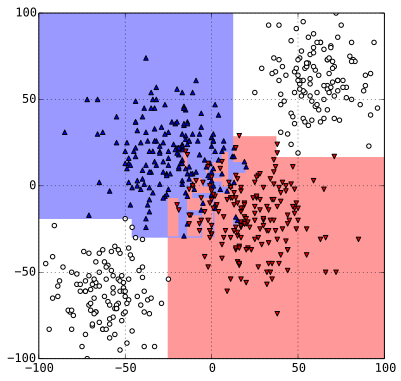
\includegraphics[width=.5\linewidth]{images/dec.plain.eps}}
\subfloat[1e-1.]{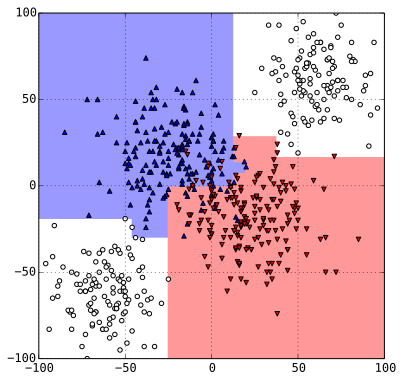
\includegraphics[width=.5\linewidth]{images/dec.prune.eps}}
\caption{region segmentation by a decision tree.\label{fig:dec.plain}}
\end{figure}

学習結果は過剰に複雑な境界線を描き、標本には忠実だが、母集団から乖離している。これを\textbf{過学習}と呼ぶ。
過学習を防ぐには、決定木の枝刈りを行うか、第\ref{sect:dec.ensem}で学ぶアンサンブル学習により\textbf{汎化性能}の改善を図る。

\section{汎化誤差の最小化\label{sect:dec.ensem}}

標本$\seq{\bm{x}_n,y_n}$から得た関数$\hat{f}(\bm{x})$と真の$f(\bm{x})$の間には\textbf{汎化誤差}が生じ、期待値を分解すると\eqref{dec.bag.E}を得る。
%
\begin{equation}
\label{eq:dec.bag.E}
\int_{\bm{x}}P(\bm{x})(y-\hat{f}(\bm{x}))^2d\bm{x} = \Var{y-f(\bm{x})} + \left(\E{\hat{f}(\bm{x})} - f(\bm{x})\right)^2 + \Var{\hat{f}(\bm{x})}.
\end{equation}

$T$個の分類器$\seq{\hat{f}_t(\bm{x})}$を\textbf{弱学習器}と称して糾合し、投票で誤差の抑制を図る手法を\textbf{アンサンブル学習}と呼ぶ。
%
\begin{equation}
\label{eq:dec.bag.f}
\hat{f}(\bm{x}) = \argmax_k \frac{1}{T} \sum_{t=1}^T \Ii{\hat{f}_t(\bm{x})=k}
\where \Ii{\hat{f}_t(\bm{x})=k} =
\begin{cases}
1 & \text{if $\hat{f}_t(\bm{x})=k$}, \\
0 & \text{if $\hat{f}_t(\bm{x})\neq k$}.
\end{cases}
\end{equation}

中でも\textbf{バギング}と呼ばれる手法では、\eqref{dec.bag.C}に示す相関を抑制することで、\eqref{dec.bag.E}の第3項の抑制を図る。
%
\begin{equation}
\label{eq:dec.bag.C}
\Var{\hat{f}(\bm{x})} = \frac{1}{T^2}\sum_{i=1}^T \sum_{j=1}^T \Cov{\Ii{f_i(\bm{x})=k},\Ii{f_j(\bm{x})=k}}.
\end{equation}

下記の\texttt{Bagging}クラスは、要素の重複を許して濃度$N$の標本を$T$通り抽出し、\eqref{dec.bag.C}の相関を抑制する。

\begin{Verbatim}{Scala}
case class Bagging[T](Y: Seq[(Seq[Int], T)], T: Int, N: Int) extends Node[T] {
	val t = Seq.fill(T)(Question(Seq.fill(N)(Y(util.Random.nextInt(Y.size)))))
	def apply(x: Seq[Int]) = t.map(_(x)).groupBy(identity).maxBy(_._2.size)._1
}
\end{Verbatim}

他方、\textbf{ブースティング}と呼ばれる手法では、弱学習器$\hat{f}_t(\bm{x})$は$\hat{f}_{t-1}(\bm{x})$が判断を誤る点を重点的に学習する。
$\hat{f}_t(\bm{x})$と$\hat{f}_{t-1}(\bm{x})$は対等でなく、その信頼度に基づく加重$\seq{w_t}$を付与され、\eqref{dec.ada.f}に示す加重投票を行う。
%
\begin{equation}
\label{eq:dec.ada.f}
\hat{f}(\bm{x}) = \argmax_k \sum_{t=1}^T w_t \Ii{\hat{f}_t(\bm{x}_n)=k}.
\end{equation}

学習の目標は、\eqref{dec.ada.E}に示す\textbf{指数誤差}の期待値を最小化する弱学習器$\seq{\hat{f}_t(\bm{x})}$と加重$\seq{w_t}$の設定にある。
%
\begin{equation}
\label{eq:dec.ada.E}
\E{\sum_{n=1}^N \exp \seq{-\frac{1}{K} \sum_{k=1}^K \Ik{k}{y_n} \Ik{k}{\hat{f}(\bm{x})}}}
\where \Ik{k}{y} =
\begin{cases}
\hfill1\hfill& \text{if $y=k$},\\
\frac{1}{1-K}& \text{if $y\neq k$}.
\end{cases}
\end{equation}

最後の弱学習器$\hat{f}_T(\bm{x})$の学習に着目し、標本の分布$P_T(\bm{x},y)$を導入して、\eqref{dec.ada.E}を\eqref{dec.ada}に変形する。
%
\begin{equation}
\label{eq:dec.ada}
\E{\sum_{n=1}^N P_T(\bm{x}_n,y_n) \exp \seq{-\frac{1}{K} \sum_{k=1}^K \Ik{k}{y_n} w_T \Ik{k}{\hat{f}_T(\bm{x}_n)}}}.
\end{equation}

\eqref{dec.ada.E}の変形の過程で現れる分布$P_T(\bm{x},y)$は、弱学習器$\hat{f}_{T-1}(\bm{x})$が判断を誤る点を重点的に学習させる。
%
\begin{equation}
\label{eq:dec.ada.P}
P_T(\bm{x}_n,y_n) = \exp \seq{-\frac{1}{K} \sum_{k=1}^K \Ik{k}{y_n} \sum_{t=1}^{T-1} w_t \Ik{k}{\hat{f}_t(\bm{x}_n)}}.
\end{equation}

\eqref{dec.ada.P}に従う標本を抽出する操作は、\textbf{ノイマンの棄却法}を利用して、下記の\texttt{Resample}クラスに実装する。

\begin{Verbatim}{Scala}
case class Resample[T](Y: Seq[(Seq[Int], T)], P: Seq[Double]) extends Node[T] {
	def reject(i: Int) = if(util.Random.nextDouble * P.max < P(i)) Y(i) else null
	val data = new collection.mutable.ArrayBuffer[(Seq[Int], T)]
	while(data.size < P.size) data += reject(util.Random.nextInt(P.size)) -= null
	val quest = Question(data)
	val error = Y.zip(P).map{case ((x, y), p) => if(quest(x) != y) p else 0}.sum
	def apply(x: Seq[Int]) = quest(x)
}
\end{Verbatim}

下記の\texttt{AdaStage}クラスは$M$個の候補$\seq{\hat{f}_{tm}(\bm{x})}$から誤差$E_t$が最小の候補を選び、弱学習器$\hat{f}_t(\bm{x})$とする。

\begin{Verbatim}{Scala}
case class AdaStage[T](Y: Seq[(Seq[Int], T)], P: Seq[Double], M: Int) extends Node[T] {
	val best = List.fill(M)(Resample(Y, P.map(_ / P.sum))).minBy(_.error)
	val W = math.log((1 / best.error - 1) * (Y.map(_._2).toSet.size - 1))
	def isOK = best.error < 0.5
	def apply(x: Seq[Int]) = best(x)
	def apply(x: Seq[Int], y: T): Double = if(best(x) == y) W else 0
	val next = Y.zip(P).map{case ((x, y), p) => p * math.exp(W - this(x, y))}
}
\end{Verbatim}

\texttt{W}は\eqref{dec.ada}を最小化する加重$W_T$であり、\eqref{dec.ada.w}で計算する。ただし、$K$はクラスの異なり数である。
%
\begin{equation}
\label{eq:dec.ada.w}
\hat{w}_T = \seq{\log \left(\frac{1}{E_T} - 1\right) + \log (K-1)} \where E_T = \sum_{n=1}^N P(\bm{x}_n,y_n) \Ii{\hat{f}_T(\bm{x}_n) \neq y_n}.
\end{equation}

下記の\texttt{AdaBoost}クラスは、弱学習器$\hat{f}_t(\bm{x})$の誤差$E_t$が$0.5$を上回るまで$\hat{f}_t(\bm{x})$を生成し、加重投票を行う。

\begin{Verbatim}{Scala}
case class AdaBoost[T](Y: Seq[(Seq[Int], T)], M: Int) extends Node[T] {
	val stages = Seq(AdaStage(Y, Y.map(_ => 1.0 / Y.size), M)).toBuffer
	while(stages.last.isOK) stages += AdaStage(Y, stages.last.next, M)
	def apply(x: Seq[Int], y: T): Double = stages.init.map(_(x, y)).sum
	def apply(x: Seq[Int]) = Y.map(_._2).distinct.maxBy(this(x, _))
}
\end{Verbatim}

\eqref{dec.ada.E}を最小化する$\hat{f}(\bm{x})$は\eqref{dec.ada.L.f}を満たす。故に、指数誤差の最小化は\eqref{dec.bag.E}の第2項を抑制する。
%
\begin{equation}
\label{eq:dec.ada.L.f}
\hat{f}(\bm{x}) = \argmin_k (K-1) \seq{\log P(y=k|\bm{x}) - \frac{1}{K} \sum_{k=1}^K \log P(y=k|\bm{x})} = \argmin_k P(y=k|\bm{x}).
\end{equation}

比較のため、\figref{dec.plain}と同じ標本を\texttt{Bagging}クラスと\texttt{AdaBoost}クラスに学習させた結果を\figref{dec.ensem}に示す。

\begin{figure}[h]
\centering
\subfloat[\texttt{Bagging}  class.]{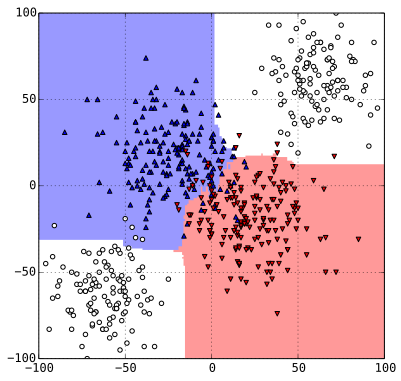
\includegraphics[width=.5\linewidth]{images/dec.bag50.eps}}
\subfloat[\texttt{AdaBoost} class.]{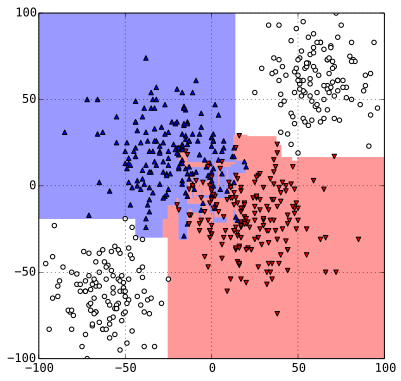
\includegraphics[width=.5\linewidth]{images/dec.ada50.eps}}
\caption{region segmentation by ensemble learning.\label{fig:dec.ensem}}
\end{figure}

\textbf{バイアスバリアンス理論}では、\eqref{dec.bag.E}の汎化誤差の第2項を\textbf{バイアス}と呼び、第3項を\textbf{バリアンス}と呼ぶ。
決定木は、バイアスが低くバリアンスが高いモデルなので、ブースティングよりもバギングが効果的である。

\section{情報源符号化と可逆圧縮\label{sect:huff}}

\chapref{dec}や\chapref{nn}には、エントロピーや\nKL 情報量などの\textbf{情報理論}に所縁のある概念が登場した。
付録\ref{sect:huff}では、情報理論を\textbf{情報源符号化}の観点から理解するため、可逆圧縮ツール\huff{}をD言語で実装する。

\begin{Verbatim}{bash}
$ ./huff encode alice.txt bob.rz
$ ./huff decode bob.rz alice.txt
\end{Verbatim}

\subsection{情報源符号化}

確率$P(s)$に従う記号$s$の系列$\seq{s}$を出力する情報源$S$に対し、記号$s$の集合$A_S$を情報源$S$の\textbf{字母}と呼ぶ。
情報源$S$の字母$A_S$から別の字母$A_C$への写像$C$を\textbf{情報源符号}と呼び、符号$C$の値$c\!\in\!C$を\textbf{符号語}と呼ぶ。

\begin{table}[h]
\centering
\caption{source coding examples.\label{tab:huff}}
\subfloat[constant length.\label{tab:huff:fix}]{
\begin{tabular}{rrrr} \toprule
$s$ & $c$ & $P(s)$ & $H(s)$ \\ \midrule
\texttt{A} & 00 & 0.5 & 1.00 \\
\texttt{B} & 01 & 0.2 & 2.32 \\
\texttt{C} & 11 & 0.2 & 2.32 \\
\texttt{D} & 10 & 0.1 & 3.32 \\ \bottomrule
\end{tabular}
}
\quad
\subfloat[variable length.\label{tab:huff:var}]{
\begin{tabular}{rrrr} \toprule
$s$ & $c$ & $P(s)$ & $H(s)$ \\ \midrule
\texttt{A} & 0   & 0.5 & 1.00 \\
\texttt{B} & 10  & 0.2 & 2.32 \\
\texttt{C} & 110 & 0.2 & 2.32 \\
\texttt{D} & 111 & 0.1 & 3.32 \\ \bottomrule
\end{tabular}
}
\end{table}

\subtabref{huff}{fix}は、符号の例である。符号語$c$の長さを\textbf{符号語長}と呼び、特に2進表記の場合に\textbf{ビット数}と呼ぶ。
特に\subtabref{huff}{fix}に挙げた\textbf{固定長符号}の場合、符号語長$L(c)$の下限は字母$A_S$の濃度の対数で決定される。
%
\begin{equation}
L(C) \ge \lceil \log_2 |A_S| \rceil = \log_2 4 = 2.
\end{equation}

記号$s$の情報量$I(s)$に応じて符号語長$L(c)$を変化させる\textbf{可変長符号}は、平均符号語長$\overline{L(C)}$を削減できる。
%
\begin{equation}
\overline{L(C)} = \sum_{s \in A_S} P(s) L(C(s)) = 0.5 \times 1 + 0.2 \times 2 + (0.2 + 0.1) \times 3 = 1.8
\end{equation}

\eqref{huf.shannon}に示すシャノンの\textbf{情報源符号化定理}は、可変長符号$C$が達成できる$\overline{L(C)}$の理論的な下限を与える。
%
\begin{equation}
\label{eq:huf.shannon}
\overline{L(C)} \geq H(P) = -\sum_{s \in A_S} P(s) \log P(s).
\end{equation}

\textbf{交差エントロピー}$H(P,Q)$は、符号$C$が想定する分布$Q(s)$が真の分布$P(s)$と異なる場合の下限を与える。
その際の余分な符号語長が\nKL 情報量$\KL{P}{Q}$であり、分布$P$と$Q$の差を測る尺度でもある。
%
\begin{equation}
\label{eq:huf.ce}
H(P,Q)
= -\sum_{s \in A_S} P(s) \log Q(s)
= -\sum_{s \in A_S} P(s) \left\{\log P(s) - \log\frac{P(S)}{Q(S)}\right\}
= H(P) + \KL{P}{Q}.
\end{equation}

現実には、符号語長$L(c)$は整数に限られ、情報源$S$の真の分布$P(s)$に従う可変長符号の実現は困難である。
実際の圧縮アルゴリズムは、\nKL 情報量の現実的な低減を目指して様々な亜種が派生している。

\subsection{ハフマン符号}

\textbf{ハフマン符号}とは、記号$s$に対して、$L(c)\!\sim\!I(s)$となる最短の符号語$c$を充てる代表的な符号化方式である。
通常、ハフマン符号は\figref{huff}に示す\textbf{ハフマン木}で表す。左右の分岐が符号語$c$の2進数の1桁に相当する。

\begin{figure}[h]
\centering
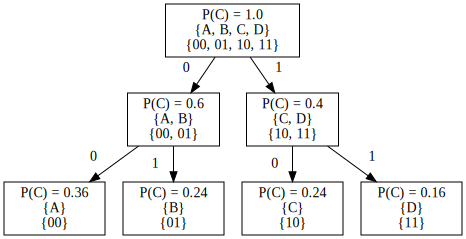
\includegraphics[width=.5\linewidth]{images/ent.codes.eps}
\caption{Huffman coding tree.\label{fig:huff}}
\end{figure}

符号語は、ハフマン木を巡回することで得られる。下記は、円周率1,000桁の符号語列の冒頭部の例である。

\begin{Verbatim}{bash}
01111110 11011100 10100010 00101101 00001100 00011001 11010001 10100110
01110011 01010110 11100011 01100101 10101110 10000011 11101000 10011100
10110011 10101110 11000111 00100011 11100001 01111110 00001010 11111100
11101100 10011001 10000010 00100111 11111110 00110111 01110011 11111010
10001110 10101111 10011001 00001110 10100011 11110111 10000101 00000111
10001010 11011110 11111110 11110100 00101010 11100001 11111001 11010001
01011010 00101001 11111111 01110111 00111011 11110001 10011100 11001101
11111100 00000011 11100000 10100100 11101111 00100000 11000100 11001111
10011010 10001110 00011011 01101111 01100000 11111010 00111001 01111110
\end{Verbatim}

但し、実際には符号語の前にハフマン木の復元に使う情報を埋め込む必要がある。以下、実装例を掲載する。

\begin{Verbatim}{dlang}
import core.bitop,std.algorithm,std.bitmanip,std.conv,std.file;
\end{Verbatim}

まず、ハフマン木を格納する方法を検討する。専用のクラスを定義しても良いが、単なる配列で十分である。
$N$種類の記号を符号化する場合、ハフマン木の枝の数は$N\!-\!1$本であるので、ノードの数は$2N\!-\!1$個となる。

\begin{Verbatim}{dlang}
size_t parent[511];
size_t child0[511];
size_t child1[511];
size_t weight[511];
\end{Verbatim}

\texttt{countSymbols}関数は、符号化前のバイト列を引数に取り、各記号の出現回数を数えて正規化した値を返す。

\begin{Verbatim}{dlang}
ubyte[256] countSymbols(ubyte[] source) {
	size_t count[256];
	foreach(sym; source) count[sym]++;
	size_t maxim = reduce!(max)(count);
	foreach(s, cnt; count) if (cnt > 0) {
		double deg = 255.0 * cnt / maxim;
		count[s] = to!ubyte(max(deg, 1));
	} else count[s] = 0;
	return to!(ubyte[256])(count);
}
\end{Verbatim}

\texttt{findRareSymbol}関数は、前掲の配列\texttt{weight}を走査して、出現頻度が最低の2個のノードの組を探索する。

\begin{Verbatim}{dlang}
size_t findRareSymbol(size_t exclusion) {
  size_t idx = exclusion;
	size_t min = size_t.max;
  foreach(i, c; weight) if(c) {
    if(i == exclusion) continue;
    if(c < min) min = c,idx = i;
  }
  return idx;
}
\end{Verbatim}

\texttt{addHuffmanTreeNode}関数は、\texttt{findRareSymbol}関数が見つけたノードの組を纏めたノードを配列に加える。

\begin{Verbatim}{dlang}
bool addHuffmanTreeNode(const size_t n) {
  size_t i = findRareSymbol(510);
  size_t j = findRareSymbol(i);
  if(i == j && i > 255) return true;
  weight[n] = weight[i] + weight[j];
  weight[i] = weight[j] = 0;
  parent[i] = parent[j] = n;
  child0[n] = i;
  child1[n] = j;
  return false;
}
\end{Verbatim}

$N$種類の記号を符号化する際は、この操作を$N\!-\!1$回だけ繰り返すことで、完全なハフマン木を構築できる。
ASCIIを符号化する際には、$N\!-\!1\!=\!255$回の反復である。下記の\texttt{createHuffmanTree}関数の通り実装した。

\begin{Verbatim}{dlang}
size_t createHuffmanTree(ubyte[] count) {
	weight[0..256] = to!(size_t[])(count);
	size_t root = 0;
	foreach(n; 256..511) {
		if(!addHuffmanTreeNode(n)) root = n;
	}
	return root;
}
\end{Verbatim}

以上で、ハフマン木を構築する処理が完成した。下記の\texttt{symbolToCodeWord}関数で、記号1件を符号化する。
これは、ハフマン木を末端から根に向け巡回することで、記号$s$に対応する符号語$c$の2進表現を取得する。

\begin{Verbatim}{dlang}
bool[] symbolToCodeWord(const size_t s) {
	bool[] code = new bool[0];
	for(long n=s; parent[n]; n=parent[n]) {
		code ~= child1[parent[n]] == n;
	}
	return code.reverse;
}
\end{Verbatim}

下記の\texttt{encode}関数は、復元時のバイト数と、各記号の出現頻度を出力したのち、符号語を順番に出力する。
なお、符号化に使ったハフマン木は復号時にも必要なので、\texttt{countSymbols}関数の返り値も冒頭に出力する。

\begin{Verbatim}{dlang}
void encode(string from, string target) {
	auto plain = cast(ubyte[]) read(from);
	createHuffmanTree(countSymbols(plain));
	ubyte[] coded = new ubyte[8];
	coded.append!(size_t)(plain.length);
	coded ~= countSymbols(plain);
	ubyte buf, i;
	foreach(s; plain) {
		foreach(b; symbolToCodeWord(s)) {
			if(b) buf |= 1; else buf &= ~1;
			if(++i % 8 != 0) buf <<= 1;
			else coded ~= buf, buf = 0;
		}
	}
	if(i % 8) coded ~= buf <<= 7 - i % 8;
	write(target, coded);
}
\end{Verbatim}

下記の\texttt{decode}関数は、符号語列を1ビットずつ走査してハフマン木を辿り、符号化前の記号列を復元する。

\begin{Verbatim}{dlang}
void decode(string from, string target) {
	auto coded = cast(ubyte[]) read(from);
	auto size = coded[0..8].peek!size_t();
	auto freq = coded[8..264];
	size_t root = createHuffmanTree(freq);
	size_t s = root;
	ubyte[] plain;
	foreach(size_t bits; coded[264..$]) {
		foreach_reverse(i; 0..8) {
			const int bit = bt(&bits, i);
			s = (bit? child1: child0)[s];
			if(s >= 256) continue;
			plain ~= to!ubyte(s), s = root;
			if(--size == 0) break;
		}
	}
	write(target, plain);
}
\end{Verbatim}

最後に、\texttt{main}関数を定義する。\huff{}の最初の引数が\texttt{encode}の場合は圧縮して、\texttt{decode}の場合は解凍する。

\begin{Verbatim}{dlang}
void main(string[] args) {
	if(args[1] == "encode") encode(args[2], args[3]);
	if(args[1] == "decode") decode(args[2], args[3]);
}
\end{Verbatim}

以上で、可逆圧縮ツール\huff{}が完成した。\dmd{}を利用する場合、下記のコマンドによりコンパイルできる。

\begin{Verbatim}{bash}
$ dmd huff -O -release -inline
\end{Verbatim}

なお、符号化したファイルの内容を確認する際には、\xxd{}等の2進ダンプのツールを利用すると便利である。

\begin{Verbatim}{bash}
$ xxd -b -g 1 -c 8 bob.rz
\end{Verbatim}

\chapter{混合正規分布と最尤推定\label{chap:gmm}}

\chapref{gmm}では、観測データ$\bm{x}$が従う何らかの確率分布$P(\bm{x})$を仮定し、分布$P(\bm{x})$の母数を求める手順を学ぶ。
単峰型の分布としては正規分布が代表的だが、\figref{gmm.model}に示す\textbf{混合正規分布}なら多峰型の分布を表現できる。

\begin{figure}[h]
\centering
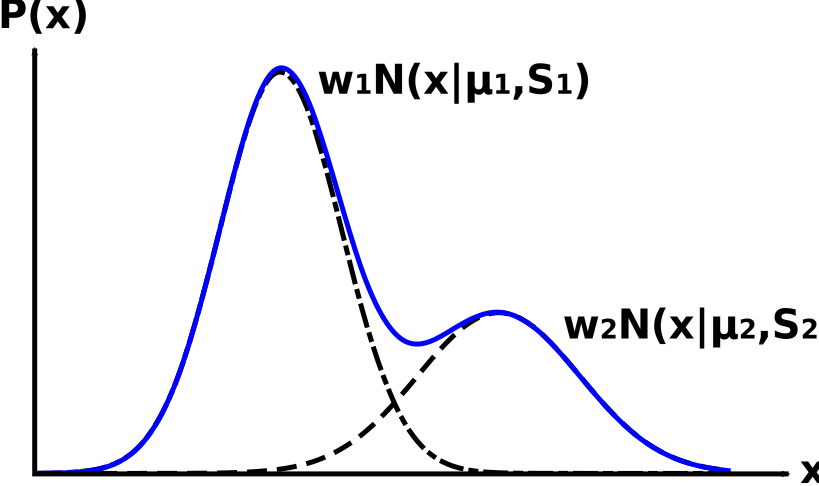
\includegraphics[width=.5\linewidth]{images/gmm.model.eps}
\caption{Gaussian mixture model.\label{fig:gmm.model}}
\end{figure}

混合正規分布は$K$個の正規分布の線型和である。変数$\bm{x}\!\in\!\mathbb{R}^D$は、確率$w_k$で正規分布$\Nd{\bm{x}|\bm{\mu}_k,S_k}$に従う。
%
\begin{equation}
\label{eq:gmm}
P(\bm{x}) = \sum_{k=1}^K w_k \Nd{\bm{x}|\bm{\mu}_k,S_k} \where\sum_{k=1}^K w_k = 1.
\end{equation}

$\bm{\mu}_k$と$S_k$は$k$番目の正規分布の平均と\textbf{分散共分散行列}である。正規分布$\Nd{\bm{x}|\bm{\mu},S}$は\eqref{gmm.gauss}で定義される。
%
\begin{equation}
\label{eq:gmm.gauss}
\Nd{\bm{x}|\bm{\mu},S} = \frac{1}{(\sqrt{2\pi})^D\sqrt{|S|}} \exp \left\{-\frac{1}{2} \trans{(\bm{x}-\bm{\mu})} S^{-1} (\bm{x}-\bm{\mu})\right\}.
\end{equation}

母数$\seq{w_k,\bm{\mu}_k,S_k}$の値を推定する前に、標本$\seq{\bm{x}_n}$を$K$個の部分集合に分類する問題を\sectref{gmm.km}で検討する。

\section{クラスタリング\label{sect:gmm.km}}

相互に近接した2点が同じ部分集合に配属されるように標本$\seq{\bm{x}_n}$を分割する操作を\textbf{クラスタリング}と呼ぶ。
直感的には、最適な部分集合$C_k$は、重心$\bm{\mu}_k$と内部の座標$\forall{}\bm{x}\!\in\!C_k$との距離の総和を最小化する筈である。
%
\begin{equation}
\label{eq:gmm.km.D}
\mathcal{D} = \sum_{n=1}^N \sum_{k=1}^K z_{nk} \|\bm{x}_n-\bm{\mu}_k\|^2.
\end{equation}

ただし、$z_{nk}$は点$\bm{x}_n$の所属を表す変数で、\eqref{gmm.km.Z.def}に定義する。$z_{nk}$は観測$\seq{\bm{x}_n}$の埒外の\textbf{潜在変数}である。
%
\begin{equation}
\label{eq:gmm.km.Z.def}
\hat{z}_{nk} =
\begin{cases}
1& \text{if $\bm{x}_n     \in C_k$}\\
0& \text{if $\bm{x}_n \not\in C_k$}.
\end{cases}
\end{equation}

最適な$\seq{z_{nk}}$と$\seq{\bm{\mu}_k}$は、反復法で求める。まず$\seq{\bm{\mu}_k}$を乱数で初期化し、次に\eqref{gmm.km.Z}で$\seq{z_{nk}}$を更新する。
%
\begin{equation}
\label{eq:gmm.km.Z}
\hat{z}_{nk} =
\begin{cases}
1& \text{if $k=   \argmin_{k}\|\bm{x}_n-\bm{\mu}_k\|^2$}\\
0& \text{if $k\neq\argmin_{k}\|\bm{x}_n-\bm{\mu}_k\|^2$}.
\end{cases}
\end{equation}

次に、\eqref{gmm.km.M}で$\seq{\bm{\mu}_k}$を更新する。以後、\eqref{gmm.km.Z}の操作と\eqref{gmm.km.M}の操作を交互に反復し、収束解を得る。
%
\begin{equation}
\label{eq:gmm.km.M}
\hat{\bm{\mu}}_k = \frac{1}{N_k} \sum_{n=1}^N z_{nk} \bm{x}_n \where N_k = \sum_{n=1}^N z_{nk}\;
\leftarrow \pdiff{\mathcal{D}}{\bm{\mu}_k} = 2\sum_{n=1}^N z_{nk} (\bm{x}_n-\bm{\mu}_k) = 0.
\end{equation}

\eqref{gmm.km.Z}\eqref{gmm.km.M}の反復で$\seq{C_k}$を求める手法を$k$-meansと呼ぶ。下記の\texttt{Kmeans}クラスは$k$-meansを実装する。

\begin{Verbatim}{Scala}
class Kmeans(X: Seq[Seq[Double]], K: Int, d: (Seq[Double],Seq[Double])=>Double) {
	val M = Array.fill(K, X.map(_.size).min)(Math.random)
\end{Verbatim}

標本$\seq{\bm{x}_n}$は引数\texttt{X}に渡す。引数\texttt{d}は距離関数であり、通常は\eqref{gmm.km.D}に従って、下記の2乗関数を与える。

\begin{Verbatim}{Scala}
	def quad(a: Seq[Double], b: Seq[Double]) = (a,b).zipped.map(_-_).map(d=>d*d).sum
\end{Verbatim}

下記の\texttt{apply}メソッドは、指定した座標$\bm{x}$に対し、\eqref{gmm.km.Z}に従って、至近の部分集合$C_k$の番号$k$を返す。

\begin{Verbatim}{Scala}
	def apply(x: Seq[Double]) = M.map(d(_,x)).zipWithIndex.minBy(_._1)._2
\end{Verbatim}

下記の\texttt{estep}メソッドは、標本$\seq{\bm{x}_n}$を部分集合$\seq{C_k}$に分配し、\eqref{gmm.km.M}に従って、重心$\seq{\bm{\mu}_k}$を計算する。

\begin{Verbatim}{Scala}
	def estep = X.groupBy(apply).values.map(c=>c.transpose.map(_.sum / c.size))
\end{Verbatim}

最後に、\eqref{gmm.km.Z}\eqref{gmm.km.M}の反復を実装する。回数は固定せずに、距離$\mathcal{D}$の収束を終了条件にすると完璧である。

\begin{Verbatim}{Scala}
	for(step<-1 to 100) (estep, M).zipped.foreach(_.copyToArray(_))
}
\end{Verbatim}

\figref{gmm.kmean}は、$K\!=\!2$の混合正規分布を\texttt{Kmeans}クラスで分割した結果で、特に黒縁の2点は重心$\seq{\bm{\mu}_k}$を表す。

\begin{figure}[h]
\centering
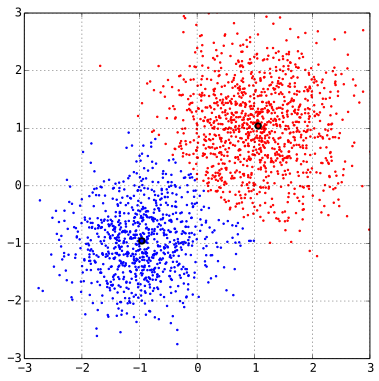
\includegraphics[width=.5\linewidth]{images/gmm.kmean.eps}
\caption{$k$-means clustering on Gaussian mixture model.\label{fig:gmm.kmean}}
\end{figure}

概してクラスタリングは、標本$\seq{\bm{x}_n}$が入力$\bm{x}$に対する出力$\bm{y}$を含まないので、\textbf{教師なし学習}に分類される。

\section{期待値最大化法\label{sect:gmm.em}}

後述の通り、$k$-meansは\sectref{gmm.em}で学ぶ期待値最大化法の特殊例であり、母数の初期値を求める際に役立つ。
\sectref{gmm.em}では、変数$\seq{z_{nk}}$を\textbf{確率変数}と見なし、重心$\bm{\mu}_k$に加えて加重$w_k$と分散$S_k$を推定する手順を学ぶ。
%
\begin{equation}
\label{eq:gmm.estep}
P(z_{nk}=1|\bm{x}_n) = \normal{k=1}{K}{w_k \Nd{\bm{x}_n|\bm{\mu}_k,S_k}} = \gamma_{nk}.
\end{equation}

\eqref{gmm.estep}に定義した$\gamma_{nk}$は、観測$\bm{x}_n$を得た後の潜在変数$z_{nk}$の確率分布を表すため、\textbf{事後確率}と呼ばれる。
以後、母数$\seq{w_k,\bm{\mu}_k,S_k}$の最尤推定の式を導出する。まず、母数の値の妥当性を担保する尤度$\mathcal{L}$を定義する。
%
\begin{equation}
\label{eq:gmm.L}
\Lk{\seq{w_k,\bm{\mu}_k,S_k}} = P(\seq{\bm{x}_n}|\seq{w_k,\bm{\mu}_k,S_k}) = \prod_{n=1}^N P(\bm{x}_n|\seq{w_k,\bm{\mu}_k,S_k}).
\end{equation}

\eqref{gmm.L}に\eqref{gmm}を代入して、\eqref{gmm.L.log}を得る。対数は、微小値の積による指数部の\textbf{アンダーフロー}を防ぐ。
%
\begin{equation}
\label{eq:gmm.L.log}
\log \Lk{\seq{w_k,\bm{\mu}_k,S_k}}
= \log\prod_{n=1}^N \sum_{k=1}^K w_k \Nd{\bm{x}_n|\bm{\mu}_k,S_k}
= \sum_{n=1}^N \log \sum_{k=1}^K w_k \Nd{\bm{x}_n|\bm{\mu}_k,S_k}.
\end{equation}

以後、尤度$\mathcal{L}$の最大化を目指す。しかし、解析的な求解は困難である。\eqref{gmm.L.m}に$\bm{\mu}_k$の偏微分の例を示す。
%
\begin{equation}
\label{eq:gmm.L.m}
\pdiff{}{\bm{\mu}_k}\log\mathcal{L} =
\pdiff{}{\bm{\mu}_k}\sum_{n=1}^N \log\sum_{k=1}^K w_k \Nd{\bm{x}_n|\bm{\mu}_k,S_k} =
\sum_{n=1}^N \gamma_{nk} S_k^{-1} (\bm{x}_n - \bm{\mu}_k).
\end{equation}

\eqref{gmm.L.m}の偏微分を0にする$\bm{\mu}_k$が、平均$\bm{\mu}_k$の推定値$\hat{\bm{\mu}_k}$となる。分散$S_k$の推定値$\hat{S_k}$も同様に計算する。
%
\begin{equation}
\label{eq:gmm.mstep.m}
\left\{
\begin{aligned}
\hat{\bm{\mu}_k} &= \frac{1}{N_k} \sum_{n=1}^N \gamma_{nk} \bm{x}_n,\\
\hat{S_k} &= \frac{1}{N_k} \sum_{n=1}^N \gamma_{nk} (\bm{x}_n - \bm{\mu}_k)\;\trans{(\bm{x}_n - \bm{\mu}_k)}.
\end{aligned}
\right\}
\where N_k = \sum_{n=1}^N \gamma_{nk}.
\end{equation}

分散$\hat{S}_k$は、変数$\bm{x}$の各次元の独立性を仮定する場合は、\eqref{gmm.mstep.s}で代用できる。$\circ$は\textbf{要素ごとの積}を表す。
%
\begin{equation}
\label{eq:gmm.mstep.s}
\hat{S_k} = \frac{1}{N_k} \left(\sum_{n=1}^N \gamma_{nk} \bm{x}_n^{\circ 2}\right) - \bm{\mu}_k^{\circ 2}.
\end{equation}

加重$w_k$の推定値$\hat{w_k}$は、\eqref{gmm}の制約条件を満たす必要があるので、\textbf{ラグランジュの未定乗数法}で求める。
%
\begin{equation}
\label{eq:gmm.mstep.w}
\hat{w_k} = \frac{N_k}{N}.
\end{equation}

事後確率$\seq{\gamma_{nk}}$が求まれば母数も求まるが、$\seq{\gamma_{nk}}$の計算に$\seq{w_k,\bm{\mu}_k,S_k}$が必要であり、求解は困難である。
そこで\textbf{補助関数法}を導入し、尤度$\mathcal{L}$の下限を与える補助関数$Q$の最大化により、間接的に$\mathcal{L}$を最大化する。
%
\begin{equation}
\log \Lk{\bm{\theta}} = \max_{\bm{\gamma}} Q(\bm{\gamma}, \bm{\theta})\;
\where \bm{\gamma} = \seq{\gamma_{nk}},\;\bm{\theta}=\seq{w_k,\bm{\mu}_k,S_k}.
\end{equation}

補助関数$Q$は、\eqref{gmm.Q}の各等式の更新を交互に反復することで最大化でき、最終的には有限な値に収束する。
%
\begin{equation}
\label{eq:gmm.Q}
\begin{aligned}
\hat{\bm{\gamma}}^{t+1} &= \argmax_{\bm{\gamma}} Q(\bm{\gamma}, \bm{\theta}), \\
\hat{\bm{\theta}}^{t+1} &= \argmax_{\bm{\theta}} Q(\bm{\gamma}, \bm{\theta}).
\end{aligned}
\end{equation}

最尤推定に補助関数法を併用し、\eqref{gmm.Q}の反復により最尤推定を行う手法を\textbf{期待値最大化法}と呼ぶ。
ここで$f(x)$を凸関数、$\seq{\gamma_n}$を正の実数列とすると、\eqref{jensen}が成立し、これを\textbf{イェンゼンの不等式}と呼ぶ。
%
\begin{equation}
\label{eq:jensen}
\sum_{n=1}^N \gamma_n f(x_n) \geq f\left(\sum_{n=1}^N \gamma_n x_n\right) \where \sum_{n=1}^N \gamma_n=1.
\end{equation}

$\log$が凹関数である点に注意して、\eqref{jensen}に\eqref{gmm.L.log}を当て嵌めると、\eqref{gmm.jensen}に示す補助関数$Q$を得る。
\eqref{gmm.Q}に関連して、補助関数$Q$を最大化する$\hat{\bm{\gamma}}$と$\hat{\bm{\theta}}$を求めると、\eqref{gmm.estep}と\eqref{gmm.mstep.m}\eqref{gmm.mstep.w}を得る。
%
\begin{equation}
\label{eq:gmm.jensen}
\log \Lk{\bm{\theta}}
\geq \sum_{n=1}^N \sum_{k=1}^K \gamma_{nk} \log \frac{w_k \Nd{\bm{x}_n|\bm{\mu}_k,S_k}}{\gamma_{nk}} = Q(\bm{\gamma}, \bm{\theta}).
\end{equation}

期待値最大化法には別の解釈もある。仮に変数$\seq{z_{nk}}$が観測可能ならば、対数尤度は\eqref{gmm.L.compl}で定義される。
実際には、変数$\seq{z_{nk}}$の真の値は観測不可能なので、変数$\seq{z_{nk}}$の事後分布に関して尤度の期待値を考える。
%
\begin{equation}
\label{eq:gmm.L.compl}
\log P(\seq{\bm{x}_n,z_{nk}}|\bm{\theta}) = \sum_{n=1}^N \sum_{k=1}^K z_{nk} \log \seq{w_k \Nd{\bm{x}_n|\bm{\mu}_k,S_k}}.
\end{equation}

\eqref{gmm.Q}や\eqref{gmm.estep}で$\bm{\gamma}$を求める操作は、\eqref{gmm.L.exp}に示す\textbf{期待対数尤度}の最新値を求める操作と等価であり、
\eqref{gmm.Q}や\eqref{gmm.mstep.m}\eqref{gmm.mstep.w}で$\bm{\theta}$を求める操作は、その期待対数尤度を極大点まで近付ける操作と等価である。
%
\begin{equation}
\label{eq:gmm.L.exp}
\E[\bm{z}]{\log P(\seq{\bm{x}_n,z_{nk}}|\bm{\theta})} = \sum_{n=1}^N \sum_{k=1}^K \gamma_{nk} \log \seq{w_k \Nd{\bm{x}_n|\bm{\mu}_k,S_k}}.
\end{equation}

これが期待値最大化法の名の由来である。
余談だが、分散をスカラー行列$\varepsilon E$とすれば$\varepsilon\!\to\!\infty$の極限で\eqref{gmm.km.elog}が成立し、更に$\gamma_{nk}\!\to\!z_{nk}$も成立する。
%
\begin{equation}
\label{eq:gmm.km.elog}
\lim_{\varepsilon\to0} \varepsilon\log \seq{w \Nd{\bm{x}|\bm{\mu},\varepsilon E}} =
\lim_{\varepsilon\to0} \seq{\varepsilon\log w - \varepsilon\frac{D}{2} \log (2\pi\varepsilon) - \frac{1}{2} \|\bm{x}-\bm{\mu}\|^2} =
-\frac{1}{2} \|\bm{x}-\bm{\mu}\|^2.
\end{equation}

従って、\eqref{gmm.km.L}が成立し、更に、期待値最大化法による\eqref{gmm.km.L}の最大化は\eqref{gmm.km.D}の最小化に帰結する。
%
\begin{equation}
\label{eq:gmm.km.L}
\varepsilon \E[\bm{z}]{\log P(\seq{\bm{x}_n,z_{nk}}|\bm{\theta})} \to -\frac{1}{2} \sum_{n=1}^N \sum_{k=1}^K z_{nk} \|\bm{x}_n-\bm{\mu}_k\|^2 + C.
\end{equation}

期待値最大化法を実装する前に$K$個の正規分布$\seq{\Nd{\bm{x}|\bm{\mu}_k,S_k}}$の混合分布を下記の\texttt{GMM}クラスに実装する。

\begin{Verbatim}{Scala}
class GMM(val D: Int, val K: Int) {
	val W = Array.fill(K)(1.0 / K)
	val M = Array.fill(K, D)(math.random)
	val S = Array.fill(K, D)(math.random)
\end{Verbatim}

配列\texttt{W}と\texttt{M}と\texttt{S}は、加重$\seq{w_k}$と平均$\seq{\bm{\mu}_k}$と分散$\seq{S_k}$である。次の\texttt{apply}メソッドは\eqref{gmm.gauss}を計算する。

\begin{Verbatim}{Scala}
	def apply(x: Seq[Double]) = for((w,m,s)<-(W,M,S).zipped) yield {
		val p = math.exp(-(x,m,s).zipped.map((x,m,s)=>(x-m)*(x-m)/s).sum/2)
		w * p / (math.pow(2 * math.Pi, .5 * m.size) * math.sqrt(s.product))
	}
}
\end{Verbatim}

下記の\texttt{EM}クラスは、期待値最大化法を実装する。標本$\seq{\bm{x}_n}$は引数\texttt{X}に、正規分布の個数は引数\texttt{K}に渡す。

\begin{Verbatim}{Scala}
class EM(X: Seq[Seq[Double]], K: Int) {
	val gmm = new GMM(X.map(_.size).min, K)
\end{Verbatim}

下記の\texttt{apply}メソッドは、事後確率$\gamma_k$の最大値を与える$k$を返す。\sectref{gmm.km}の\texttt{apply}メソッドに相当する。

\begin{Verbatim}{Scala}
	def apply(x: Seq[Double]) = gmm(x).toSeq.zipWithIndex.maxBy(_._1)._2
\end{Verbatim}

次にM-射影を実装する。\eqref{gmm.mstep.w}\eqref{gmm.mstep.m}\eqref{gmm.mstep.s}に従って母数$\seq{w_k,\bm{\mu}_k,S_k}$を更新し、\eqref{gmm.L.log}の尤度を返す。

\begin{Verbatim}{Scala}
	def mstep(P: Seq[Seq[Double]]): Double = {
		for(k<-0 until K) gmm.W(k) = P(k).sum / X.size
		val m1 = P.map((_,X).zipped.map((p,x)=>x.map(x=>p*x*1)).transpose)
		val m2 = P.map((_,X).zipped.map((p,x)=>x.map(x=>p*x*x)).transpose)
		for(k<-0 until K; d<-0 until gmm.D) {
			gmm.M(k)(d) = m1(k)(d).sum / P(k).sum
			gmm.S(k)(d) = m2(k)(d).sum / P(k).sum - math.pow(gmm.M(k)(d), 2)
		}
		X.map(x=>math.log(gmm(x).sum)).sum
	}
\end{Verbatim}

\texttt{mstep}メソッドの引数は、標本$\seq{\bm{x}_n}$の事後確率$\seq{\gamma_{nk}}$である。これは、\eqref{gmm.estep}に従って求める。
下記は、期待値最大化を交互に反復する。回数を固定せずに、尤度の収束を目安にすると実用的である。

\begin{Verbatim}{Scala}
	for(step <- 1 to 100) mstep(X.map(gmm(_)).map(p=>p.map(_/p.sum)).transpose)
}
\end{Verbatim}

\figref{gmm.train}は、\figref{gmm.kmean}と同じ標本を\texttt{EM}クラスで学習した結果で、等高線は、混合正規分布の密度関数を示す。
特に、\subref{fig:gmm.train:dense}は密度関数の\textbf{ヒートマップ}を表す。また、\subref{fig:gmm.train:class}は混合正規分布によるクラスタリングの結果である。

\begin{figure}[h]
\centering
\subfloat[density map.\label{fig:gmm.train:dense}]{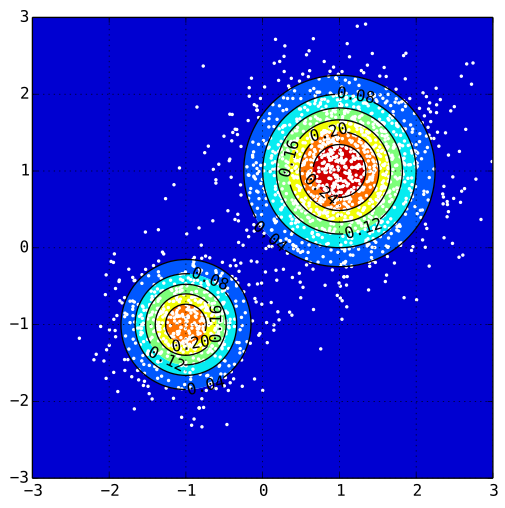
\includegraphics[width=.5\linewidth]{images/gmm.dense.eps}}
\subfloat[cluster map.\label{fig:gmm.train:class}]{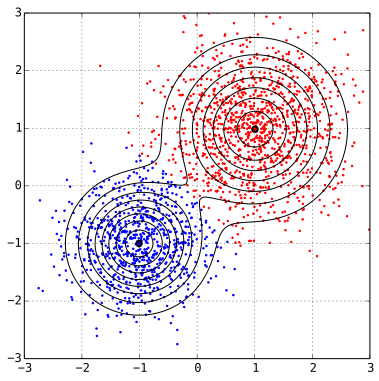
\includegraphics[width=.5\linewidth]{images/gmm.class.eps}}
\caption{expectation maximization on a Gaussian mixture model.\label{fig:gmm.train}}
\end{figure}

\figref{gmm.kmean}に比べ、正規分布が接する谷間に位置する標本は、正規分布の等高線を正しく反映した分類になる。

\chapter{潜在的ディリクレ配分法\label{chap:topic}}

\chapref{topic}では、観測データの生成過程を確率変数の因果関係などの連鎖で表現する\textbf{グラフィカルモデル}を学ぶ。
自然言語処理に焦点を当て、百科事典の記事を訓練データに使う。まず、XMLの\textbf{ダンプデータ}を入手する。

\begin{Verbatim}{bash}
$ wget https://dumps.wikimedia.org/jawiki/latest/jawiki-latest-abstract.xml
\end{Verbatim}

次に、\href{https://github.com/scala/scala-xml}{ScalaでXML文書を操作するAPI}を利用して、記事の題名と本文を抽出し、適当な配列に格納する。

\begin{Verbatim}{Scala}
val docs = scala.xml.XML.loadFile("jawiki-latest-abstract.xml") \\ "doc"
val data = Map(docs.map(d => (d\"title").text->(d\"abstract").text): _*)
\end{Verbatim}

記事には、文章を単語列に分解する\textbf{形態素解析}を予め施す。形態素解析器は、\href{http://github.com/lucene-gosen/lucene-gosen}{Lucene~GoSen}が便利だろう。

\begin{Verbatim}{Scala}
val gosen = net.java.sen.SenFactory.getStringTagger(null)
val words = gosen.analyze(data("Wikipedia: Scala"), new ArrayList[Token]())
\end{Verbatim}

助詞や助動詞や接続詞など\textbf{機能語}は、機械学習の際には無用のため、形態素解析の段階での排除を推奨する。
\eqref{nbc.tf.idf}に示す\textit{tf-idf}を指標に、特定の記事$d$で高頻度だが、他の記事で低頻度な単語$t_d$を残す方法もある。
%
\begin{equation}
\label{eq:nbc.tf.idf}
\mathrm{tf\,idf}(t_d \in d,d \in D) = \mathrm{tf}(t_d,d) \mathrm{idf}(t_d,D)\;
\where\left\{
\begin{aligned}
\mathrm{tf}(t_d,d) &= \log \biggl(1+\frac{N_{t_dd}}{\sum_t N_{td}}\biggr) \\
\mathrm{idf}(t,D) &= \log \frac{|D|}{|\seq{d: t \in d}|}
\end{aligned}
\right.
\end{equation}
%
ただし、$N_{td}$は文書$d$に単語$t$が出現する回数である。また、\eqref{nbc.tf.idf}の対数は、$\mathrm{tf}$と$\mathrm{idf}$の変動を抑制する。

\section{単純ベイズ分類器\label{sect:topic.nbc}}

\sectref{topic.nbc}で学ぶ\textbf{単純ベイズ分類器}は、単語$w_n$の列である文書$d$が、話題$c$から生成された確率を推定する。
%
\begin{equation}
\label{eq:nbc.pdc}
P(d|c) = P(w_1,\dots,w_{N_d}|c) = \prod_{n=1}^{N_d} P(w_n|c).
\end{equation}

\eqref{nbc.pdc}の$P(d|c)$は、\textbf{観測変数}たる文書$d$が潜在変数たる話題$c$から生成された場合の、仮説の尤度を表す。
単語の\textbf{共起}を考慮すると\eqref{nbc.pwc}になるが、寧ろ独立性に拘る\eqref{nbc.pdc}は、この分類器の単純たる理由である。
%
\begin{equation}
\label{eq:nbc.pwc}
P(w_1,\dots,w_{N_d}|c) = \prod_{n=1}^{N_d} P(w_n|c,w_1,...,w_{n-1}).
\end{equation}

文書$d$を生成した話題$\hat{c}_d$を推測する方法を検討する。直感的には、話題$\hat{c}_d$は確率$P(c|d)$の最大値を与える。
%
\begin{equation}
\label{eq:nbc.pcd}
\hat{c}_d = \argmax_{c \in C} P(c|d).
\end{equation}

確率$P(d)$が話題$c$に対し独立である点に留意して、\eqref{nbc.pcd}に\textbf{ベイズの定理}を適用すると、\eqref{nbc.pcd.bayes}を得る。
%
\begin{equation}
\label{eq:nbc.pcd.bayes}
\hat{c}_d = \argmax_{c \in C} \frac{P(d|c)P(c)}{P(d)} = \argmax_c P(d|c)P(c).
\end{equation}

独立性を仮定した\eqref{nbc.pdc}を\eqref{nbc.pcd.bayes}に代入すると、\eqref{nbc.pcd.words}を得る。話題を判定する際は、\eqref{nbc.pcd.words}を使う。
%
\begin{equation}
\label{eq:nbc.pcd.words}
\hat{c}_d = \argmax_{c \in C} P(c) \prod_{n=1}^{N_d} P(w_n|c).
\end{equation}

なお、確率$P(w|c)$は未知の単語$w$に対して$0$になる。対策として、\eqref{nbc.smooth}の\textbf{ラプラス平滑化}で補正する。
\eqref{nbc.smooth}の確率$P(w)$は未知語$w$の\textbf{事前確率}を、確率$P(w|c)$は訓練データを学習した後の事後確率を表す。
%
\begin{equation}
\label{eq:nbc.smooth}
P(w|c) = \frac{N_{wc}+1}{\sum_{w\in V} (N_{wc}+1)}\;
\leftarrow w \sim P(w) = \mathrm{Uniform}(V) = \frac{1}{|V|}.
\end{equation}

下記の\texttt{NaiveBayes}クラスは、観測$d$を得て潜在変数$c$の事後確率$P(d|c)$を最大化する話題$\hat{c}_d$を推定する。
型引数\texttt{W}と\texttt{C}は単語と話題を表す。引数\texttt{docs}と\texttt{cats}には、文書$\seq{d_i}$と話題$\seq{c_i}$を同じ順番に並べて渡す。

\begin{Verbatim}{Scala}
class NaiveBayes[W,C](docs: Seq[Seq[W]], cats: Seq[C]) {
	val N = scala.collection.mutable.Map[(W,C),Double]().withDefaultValue(0)
\end{Verbatim}

下記の配列\texttt{P}は、話題$c$の事前確率$P(c)$を保持する。単に、訓練データで話題$\seq{c}$が出現した頻度である。

\begin{Verbatim}{Scala}
	val P = cats.groupBy(c=>c).map{case (c,s)=>c->s.size.toDouble/docs.size}
\end{Verbatim}

次に、単語$w$と話題$c$の共起の回数$N_{wc}$を配列\texttt{N}に格納する。配列\texttt{N}は未知語$w$に対して$N_{wc}\!=\!0$を返す。

\begin{Verbatim}{Scala}
	for((d,c)<-(docs,cats).zipped; w<-d) N(w,c) += 1
\end{Verbatim}

\texttt{Pwc}メソッドは、単語$w$を観測した場合の、その原因たる話題$c$の尤度$P(w|c)$を\eqref{nbc.smooth}に従って計算する。

\begin{Verbatim}{Scala}
	def Pwc(w: W, c: C) = (N(w,c)+1) / docs.flatten.distinct.map(N(_,c)+1).sum
\end{Verbatim}

\texttt{Pcd}メソッドは、文書$d$を観測した際の、その原因たる話題$c$の事後確率$P(c|d)$を\eqref{nbc.pcd.words}により計算する。

\begin{Verbatim}{Scala}
	def Pcd(c: C, d: Seq[W]) = math.log(P(c)) + d.map(w=>math.log(Pwc(w,c))).sum
\end{Verbatim}

最後に\texttt{apply}メソッドを定義する。未知の文書$d$に対し、事後確率$P(c|d)$を最大化する話題$\hat{c}_d$を推定する。

\begin{Verbatim}{Scala}
	def apply(d: Seq[W]) = cats.distinct.maxBy(Pcd(_, d))
}
\end{Verbatim}

\subfigref{nbc.jmap}{2}は、固有名詞を特徴量として東日本と西日本の記事を学習し、46都道府県を分類した結果である。
同様に、北海道と東北、関東と中部、近畿と中国、四国に九州の8地方に分類した結果を\subfigref{nbc.jmap}{8}に示す。

\begin{figure}[h]
\centering
\subfloat[2-regional division.\label{fig:nbc.jmap:2}]{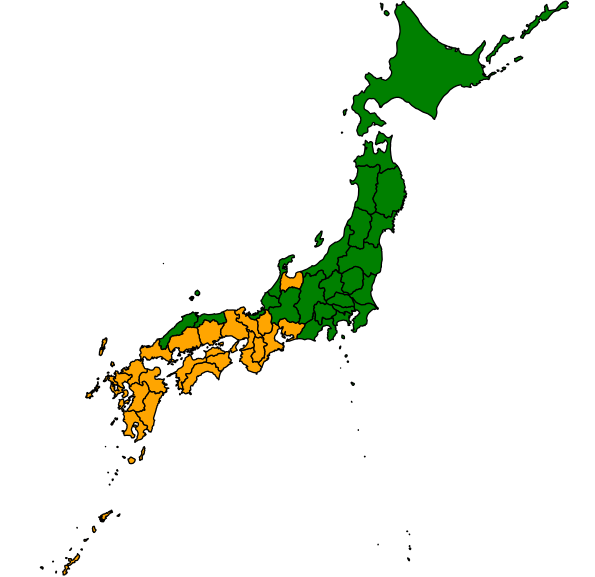
\includegraphics[width=.5\linewidth]{images/nbc.jmap2.eps}}
\subfloat[8-regional division.\label{fig:nbc.jmap:8}]{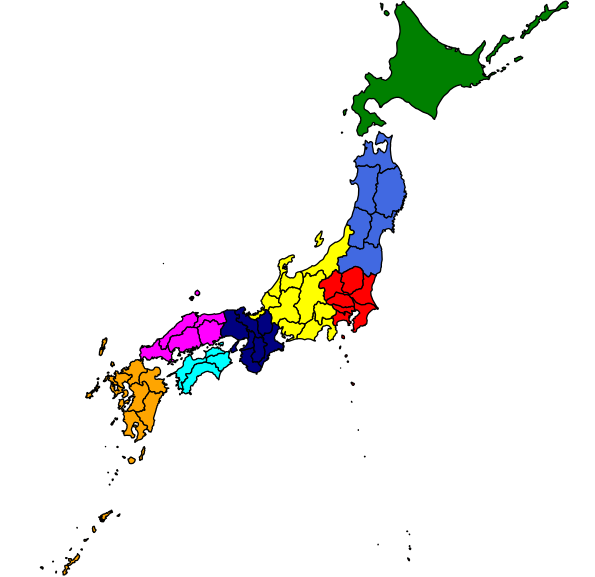
\includegraphics[width=.5\linewidth]{images/nbc.jmap8.eps}}
\caption{Japanese map division into regions based on classification of Wikipedia pages.\label{fig:nbc.jmap}}
\end{figure}

\section{単語の話題の推定\label{sect:topic.lda}}

\sectref{topic.lda}で学ぶ\textbf{潜在的ディリクレ配分法}は、話題に応じて単語の意味が変化する複雑な言語モデルを扱える。
実際の自然言語の文では、短文でも複数の話題に言及し得るので、単語と意味を区別して考える必要がある。

\begin{description}
\item[例文]\textit{I wrote a \textcolor{red}{Java} program drinking a cup of \textcolor{blue}{Java} coffee.}
\end{description}

\figref{lda.model}に示す通り、複雑な言語モデルは単語$w$や話題$z$を始め、複数の確率変数の依存関係で表現される。

\begin{figure}[h]
\centering
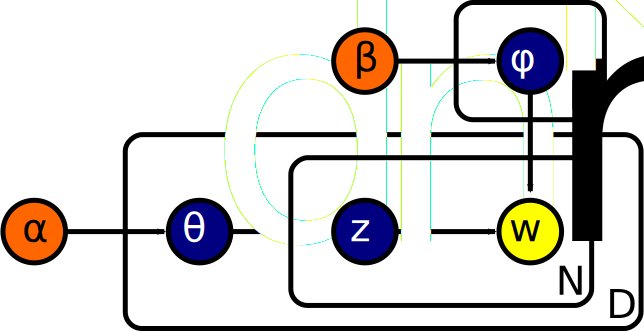
\includegraphics[width=.5\linewidth]{images/lda.model.eps}
\caption{latent Dirichlet allocation model.\label{fig:lda.model}}
\end{figure}

文書$d\!\in\!D$に出現する$n$番目の単語$w_{dn}$の話題を変数$z_{dn}$で表す。両変数は\eqref{lda.pw_z}の\textbf{多項分布}に従う。
ただし、$V$は語彙量を、$K$は話題の数を表し、$N_v\in{}\seq{0,1}$と$N_k\in{}\seq{0,1}$は単語$v$と話題$k$の出現を表す。
%
\begin{equation}
\label{eq:lda.pw_z}
\begin{aligned}
w_{dn} &\sim P(w|z) = \prod_{v=1}^V \phi_{zv}^{N_v} = \Md{\bm{\phi}_z} \where \sum_{v=1}^V N_v = 1,\\
z_{dn} &\sim P(z|d) = \prod_{k=1}^K \theta_{dk}^{N_k} = \Md{\bm{\theta}_d} \where \sum_{k=1}^K N_k = 1.
\end{aligned}
\end{equation}
%
$\phi_{zv}$は話題$z$が単語$v$を生起する確率$P(v|z)$を表し、$\theta_{dk}$は文書$d$が話題$k$を生起する確率$P(k|d)$を表す。
単語$w$と文書$d$の結合確率は\eqref{lda.pw_d}で与える。話題$z$は\textbf{潜在変数}で観測の埒外にあるので、周辺化する。
%
\begin{equation}
\label{eq:lda.pw_d}
P(w,d) = P(d) \sum_{z=1}^K P(w|z) P(z|d) = \int_z \phi_z(w) \theta_d(z) dz.
\end{equation}
%
観測された文書$d$を的確に表す母数$\phi_z$や母数$\theta_d$を推定する場合は、\eqref{lda.like}の尤度関数の極値を探索する。
%
\begin{equation}
\label{eq:lda.like}
\Lk{\phi_z,\theta_d} = P(\bm{w}_d|\phi_z,\theta_d) = \prod_{n=1}^{N_d} \int_z \phi_z(w_{dn}) \theta_d(z) dz.
\end{equation}
%
ただし、母数$\theta_d$の個数は文書の量に比例し、膨大な数になるため、単なる最尤推定では過学習を頻発する。
対策として\textbf{ベイズ推定}を導入し、文書$d$を観測した後の母数$\theta_d$や母数$\phi_z$の分布を\textbf{事後分布}として計算する。
%
\begin{equation}
\label{eq:lda.B}
P(\phi_z,\theta_d|\bm{w}_d)
= \frac{P(\bm{w}_d|\phi_z,\theta_d)P(\phi_z,\theta_d)}{P(\bm{w}_d)}
\propto P(\bm{w}_d|\phi_z,\theta_d)P(\phi_z,\theta_d).
\end{equation}
%
\eqref{lda.B}の$P(\phi_z,\theta_d)$を\textbf{事前分布}と呼び、文書$d$を観測する前に予想された母数$\phi_z$や母数$\theta_d$の分布を表し、
過学習を抑える働きを持つ。事後分布は尤度と事前分布の積に比例し、最適な母数は事後確率を最大化する。
%
\begin{equation}
\begin{aligned}
\hat{\phi}_z &= \argmax_{\phi_z} P(\phi_z,\theta_d|\bm{w}_d),\\
\hat{\theta}_d &= \argmax_{\theta_d} P(\phi_z,\theta_d|\bm{w}_d).
\end{aligned}
\end{equation}
%
なお、\eqref{lda.B}は、1件の文書を観測する場合を想定した。文書が複数ある場合には、\eqref{lda.B.D}を適用する。
%
\begin{equation}
\label{eq:lda.B.D}
P(\phi_z,\theta_1,...,\theta_D|\bm{w}) \propto P(\phi_z,\theta_1,...,\theta_D) \prod_{d=1}^D P(\bm{w}_d|\phi_z,\theta_d).
\end{equation}
%
\eqref{lda.B.D}は、文書$d_t$を観測した後の事後分布を事前分布として次の文書$d_{t+1}$を学習する連鎖の様子を表す。
連鎖を容易にする目的から、事前分布は\eqref{lda.dir}の\textbf{ディリクレ分布}で定義する。$\Gd{z}$は\textbf{ガンマ関数}である。
%
\begin{equation}
\label{eq:lda.dir}
\Dd{\bm{\theta}|\bm{\alpha}} = \frac{\Gd{\sum_{k=1}^K \alpha_k}}{\prod_{k=1}^K \Gd{\alpha_k}} \prod_{k=1}^K \theta_k^{\alpha_k-1}\;
\where \Gd{z} = \int_0^\infty t^{z-1} e^{-t} dt.
\end{equation}
%
\eqref{lda.pw_z}より、\eqref{lda.like}の尤度は多項分布を描くが、\eqref{lda.conj}より、事後確率もディリクレ分布に従う。
%
\begin{equation}
\label{eq:lda.conj}
\Dd{\bm{\theta}|\bm{n}+\bm{\alpha}} \propto \Md{\bm{n}|\bm{\theta}} \Dd{\bm{\theta}|\bm{\alpha}}.
\end{equation}
%
\eqref{lda.conj}の性質により、事前確率は事後確率と共通の確率密度関数で定義でき、これを\textbf{共役事前分布}と呼ぶ。
%
\begin{equation}
\label{eq:lda.pri}
\begin{aligned}
\phi_k & \sim \Dd{\phi|\bm{\beta}},\\
\theta_d & \sim \Dd{\theta|\bm{\alpha}}.
\end{aligned}
\end{equation}
%
母数$\phi_k$と母数$\theta_d$の事前分布を\eqref{lda.pri}に設定し、\eqref{lda.B}のベイズ推定に組み込むと、\eqref{lda.B.2}を得る。
%
\begin{equation}
\label{eq:lda.B.2}
P(\bm{\phi},\bm{\theta}|\bm{w},\bm{\alpha},\bm{\beta})
\propto 
\prod_{k=1}^K \Dd{\phi_k|\bm{\beta}} 
\prod_{d=1}^D \Dd{\theta_d|\bm{\alpha}} 
\prod_{n=1}^{N_d} \int_z \phi_z(w_{dn}) \theta_d(z) dz.
\end{equation}

\eqref{lda.B.2}の事後確率を最大化する点を微分により求めれば、母数$\phi_k$や母数$\theta_d$の具体的な数値が得られるが、
微分は困難である。そこで、話題$z_{dn}$の標本を近似的に生成し、\eqref{lda.map}で母数を計算する方針を検討する。
%
\begin{equation}
\label{eq:lda.map}
\begin{aligned}
\hat{\phi}_{kv} &= \frac{N_{kv} + \beta_v}{\sum_{v=1}^V \left(N_{kv} + \beta_v\right)},\\
\hat{\theta}_{dk} &= \frac{N_{dk} + \alpha_k}{\sum_{k=1}^K \left(N_{dk} + \alpha_k\right)}.
\end{aligned}
\end{equation}
%
ただし、$N_{kv}$は話題$k$で単語$v$が出現した回数を表し、$N_{dk}$は文書$d$で話題$k$の単語が出現した回数を表す。
時刻$t$の標本$\seq{z_{dn}^t}$は、\eqref{lda.gibbs}の\textbf{提案分布}に従う乱数により生成する。これを\textbf{ギブスサンプリング}と呼ぶ。
%
\begin{equation}
\label{eq:lda.gibbs}
\forall z_{dn}^t \sim P(z_{dn}|z_{11}^t,...,z_{dn-1}^t,z_{dn+1}^{t-1},...,z_{DN_D}^{t-1}).
\end{equation}
%
変数$\phi_z$と変数$\theta_d$も潜在変数なので、本来は標本に含むべきであるが、\eqref{lda.col}の周辺化により除去できる。
%
\begin{equation}
\label{eq:lda.col}
P(\bm{z},\bm{w}|\bm{\alpha},\bm{\beta}) =
\left(\prod_{k=1}^K \int \Dd{\phi_k|\bm{\beta}} \prod_{d=1}^D \prod_{n=1}^{N_d} \phi_{z_{dn}}\!(w_{dn})\;d\phi_k\right)\!
\left(\prod_{d=1}^D \int \Dd{\theta_d|\bm{\alpha}} \prod_{n=1}^{N_d} \theta_d(z_{dn})\;d\theta_d\right).
\end{equation}
%
詳細は省略するが、\textbf{ベータ関数}の積分が出現する点に注目しつつ、\eqref{lda.col}を変形すると、\eqref{lda.pz}を得る。
%
\begin{equation}
\label{eq:lda.pz}
P(\bm{z},\bm{w}|\bm{\alpha},\bm{\beta}) =
\prod_{k=1}^K \left\{
\frac{\Gd{\sum_{v=1}^V\beta_v}}{\prod_{v=1}^V\Gd{\beta_v}}
\frac{\prod_{v=1}^V\Gd{N_{kv}+\beta_v}}{\Gd{N_k+\sum_{v=1}^V\beta_v}}
\right\}
\prod_{d=1}^D \left\{
\frac{\Gd{\sum_{k=1}^K\alpha_k}}{\prod_{k=1}^K\Gd{\alpha_k}}
\frac{\prod_{k=1}^K\Gd{N_{dk}+\alpha_k}}{\Gd{N_d+\sum_{k=1}^K\alpha_k}}
\right\}.
\end{equation}
%
\eqref{lda.pz}で単語$w_{dn}$と話題$z_{dn}$に依存する部分を\eqref{lda.gibbs}の条件付き分布に代入すると、\eqref{lda.gibbs.2}を得る。
ただし、\eqref{lda.gibbs.2}で、$\bm{w}^{\cancel{dn}}$は単語$w_{dn}$を除外した単語の列であり、$\bm{z}^{\cancel{dn}}$は$\bm{w}^{\cancel{dn}}$に対応する話題の列である。
%
\begin{equation}
\label{eq:lda.gibbs.2}
P(z_{dn}|\bm{z}^{\cancel{dn}}) \propto
P(z_{dn}=k,w_{dn}=v,\bm{z}^{\cancel{dn}},\bm{w}^{\cancel{dn}}|\bm{\alpha},\bm{\beta}) \propto
\frac{N_{kv}^{\cancel{dn}} + \beta_v}{N_k^{\cancel{dn}} + \sum_{v=1}^V \beta_v}
\frac{N_{dk}^{\cancel{dn}} + \alpha_k}{N_d^{\cancel{dn}} + \sum_{k=1}^K \alpha_k}.
\end{equation}
%
\eqref{lda.gibbs.2}の提案分布に従う標本生成を何度も反復すれば、最終的に、標本$\bm{z}$は真の分布に収束する筈である。
下記の\texttt{LDA}クラスは、潜在的ディリクレ配分法を実装する。引数\texttt{docs}に文書の題名と単語列の配列を渡す。

\begin{Verbatim}{Scala}
class LDA[W,D](docs: Map[D, Seq[W]], K: Int, a: Double = 0.1, b: Double = 0.01) {
\end{Verbatim}

引数\texttt{K}は話題の個数で、引数\texttt{a}と\texttt{b}は$\forall a_k\!=\!a,\forall b_v\!=\!b$を仮定した\textbf{対称ディリクレ分布}の母数$\alpha$と$\beta$である。
\texttt{LDA}クラス内に、単語$w_{dn}$を包む\texttt{Word}クラスを実装する。乱数で初期化される変数\texttt{z}は、話題$z_{dn}$を表す。

\begin{Verbatim}{Scala}
	case class Word(v: W, var z: Int = util.Random.nextInt(K))
\end{Verbatim}

配列\texttt{W}は集合$\seq{w_{dn},z_{dn}}$に相当する。文書$d$と位置$n$を索引として\texttt{Word}クラスのインスタンスを管理する。

\begin{Verbatim}{Scala}
	val W = docs.mapValues(_.map(Word(_)).toArray)
\end{Verbatim}

配列\texttt{V}は語彙$V$の要素$v\!\in\!V$を索引として集合$\seq{w_{dn},z_{dn}}$を管理する。変数$N_{kv}$の値を計算する際に使う。

\begin{Verbatim}{Scala}
	val V = W.flatMap(_._2).groupBy(_.v)
\end{Verbatim}

下記の\texttt{Ndk}メソッドは\eqref{lda.map}の変数$N_{dk}$に相当し、文書$d$に含まれる話題$k$の単語の出現回数を数える。

\begin{Verbatim}{Scala}
	def Ndk(d: D) = 0.until(K).map(k=>W(d).count(_.z==k) + a)
\end{Verbatim}

\texttt{Nkv}メソッドは\eqref{lda.map}の変数$N_{kv}$に相当し、単語の列$\seq{w_{dn}}$の部分集合$\seq{w_{dn}\!=\!v,z_{dn}\!=\!k}$の濃度を返す。

\begin{Verbatim}{Scala}
	def Nkv(v: W) = 0.until(K).map(k=>V(v).count(_.z==k) + b)
\end{Verbatim}

配列\texttt{NkV}は$N_{kv}$を$V$全体に渡って合計した値である。実行効率の都合から、関数ではなく配列で実装した。

\begin{Verbatim}{Scala}
	val NkV = V.keys.map(Nkv).reduce((_,_).zipped.map(_+_)).toArray
\end{Verbatim}

次に、\eqref{lda.gibbs}に従う乱数で標本$\seq{z_{dn}^t}$を更新する処理を記述する。この処理は、収束まで何度も繰り返す。

\begin{Verbatim}{Scala}
	for(step<-1 to 1000; d<-docs.keys; (w,n)<-docs(d).zipWithIndex) {
		NkV(W(d)(n).z) -= 1
		W(d)(n).z = -1
		val S = (Nkv(w), Ndk(d), NkV).zipped.map(_*_/_).scan(.0)(_+_)
		val r = util.Random.nextDouble * S.last
		W(d)(n).z = S.tail.indexWhere(_ >= r)
		NkV(W(d)(n).z) += 1
	}
\end{Verbatim}

\texttt{apply}メソッドは、文書$d$で支配的な話題を探す。未知の文書には適用できず、専らクラスタリングに使う。

\begin{Verbatim}{Scala}
	def apply(d: D) = 0.until(K).maxBy(Ndk(d)(_))
}
\end{Verbatim}

固有名詞を特徴量として46都道府県の記事を\texttt{LDA}クラスで学習し、色を塗り分けた結果を\figref{lda.jmap}に示す。

\begin{figure}[h]
\centering
\subfloat[3-regional division.]{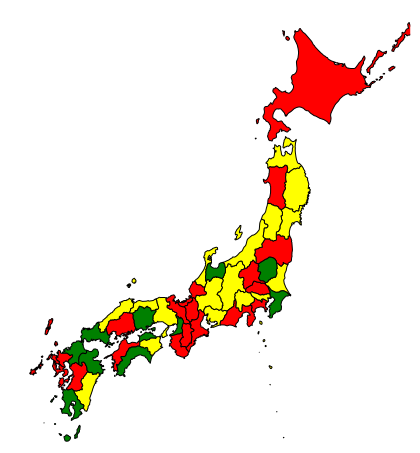
\includegraphics[width=.5\linewidth]{images/lda.jmap3.eps}}
\subfloat[5-regional division.]{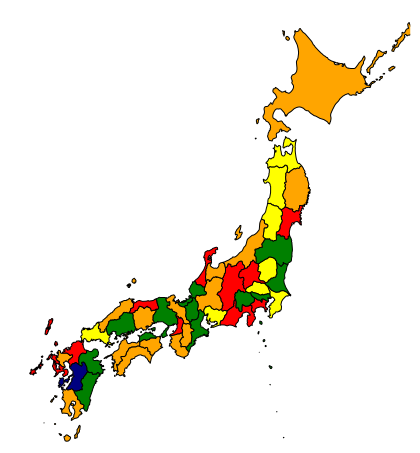
\includegraphics[width=.5\linewidth]{images/lda.jmap5.eps}}
\caption{Japanese map division into regions based on clustering of Wikipedia pages.\label{fig:lda.jmap}}
\end{figure}

教師なし学習であるため\sectref{topic.nbc}と比べて分類結果の評価は難しく、変数$N_{kv}$を詳細に解析する必要がある。

\chapter{ニューラルネットワーク\label{chap:nn}}

\textbf{ニューラルネットワーク}は神経系を模倣した計算模型であり、神経細胞に相当する単位を\textbf{ニューロン}と呼ぶ。

\begin{figure}[h]
\centering
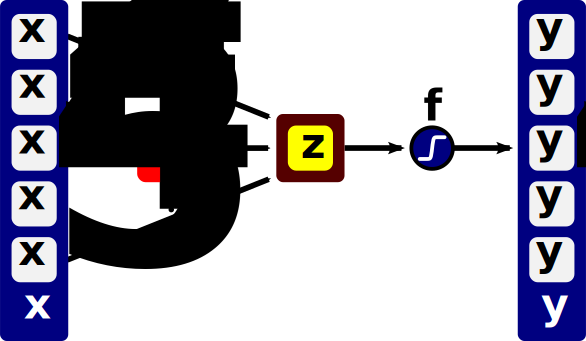
\includegraphics[width=.5\linewidth]{images/slp.model.eps}
\caption{a neuron.\label{fig:slp.model}}
\end{figure}

細胞は$D$本の樹状突起で信号$\bm{x}$を受容し、加重$\bm{w}$で合計した後、\textbf{活性化関数}$f$の値を軸索末端で放出する。
%
\begin{equation}
\label{eq:nn.neuron}
y = f(z) = f(\bm{w} \cdot \bm{x}) = f\left(\sum_{d=1}^D w_d x_d\right).
\end{equation}
%
関数$f$は、神経細胞が興奮する閾値に相当する。$f$が恒等関数$f_\mathrm{id}(z)\!=\!z$の場合、\eqref{nn.neuron}は線型回帰になる。
他方、関数$f$を階段関数や\eqref{nn.sigm}の\textbf{シグモイド関数}で実装すると、\eqref{nn.neuron}は$y\!\in\!\seq{0,1}$の2値分類になる。
%
\begin{equation}
\label{eq:nn.sigm}
\sigm(z) = \frac{1}{1 + e^{-z}} = \frac{1}{2}\tanh\frac{z}{2} + \frac{1}{2}.
\end{equation}

他にも\subfigref{slp}{acfun}に示す$\mathrm{tanh}$関数やReLU関数が存在し、回帰やクラス分類など用途に応じて選択できる。
\subfigref{slp}{judge}は、論理和を$f=\sigm$の分類器で学習した結果である。直線$f(\bm{x})\!=\!0.5$はクラスの境界を表す。

\begin{figure}[h]
\centering
\subfloat[activation functions.\label{fig:slp:acfun}]{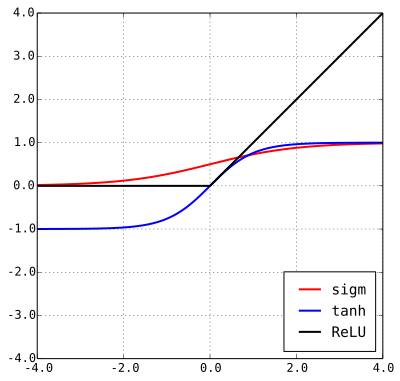
\includegraphics[width=.5\linewidth]{images/slp.acfun.eps}}
\subfloat[OR learned by neuron.\label{fig:slp:judge}]{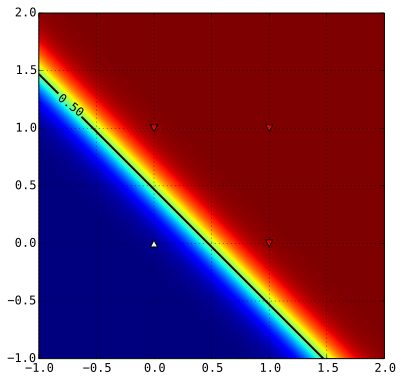
\includegraphics[width=.5\linewidth]{images/slp.judge.eps}}
\caption{neuron mechanism.\label{fig:slp}}
\end{figure}

分類器としてのニューロンは線型分類器と呼ばれ、境界が超平面になる\textbf{線型分離可能}な問題のみ学習できる。

\section{誤差逆伝播法\label{sect:nn.mlp}}

\figref{mlp.model}は、ニューロンの多層化により非線型な回帰問題や分類問題に対応した\textbf{多層パーセプトロン}である。
左端で信号$\bm{x}_1$を受容する層を\textbf{入力層}、右端で信号$\bm{x}_3$を出力する層を{\bf 出力層}と呼び、その間を{\bf 隠れ層}と呼ぶ。

\begin{figure}[h]
\centering
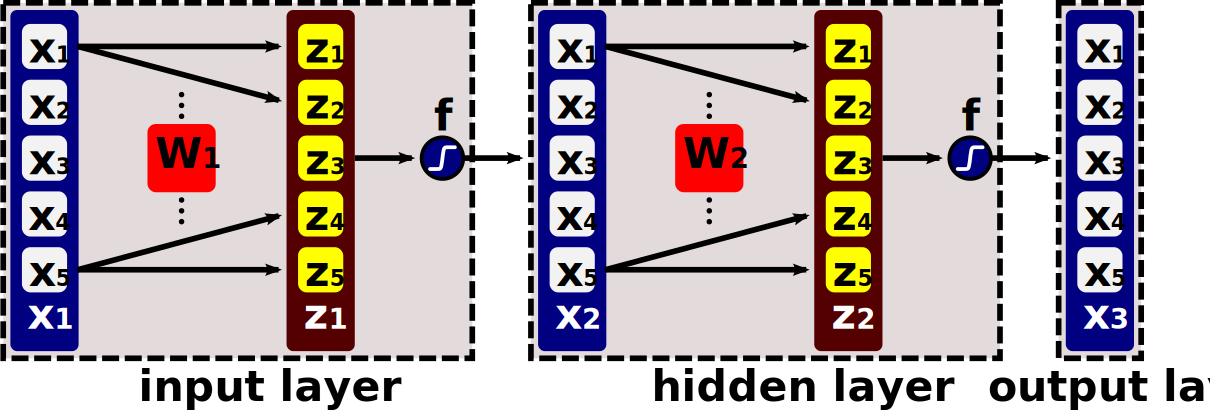
\includegraphics[width=.5\linewidth]{images/mlp.model.eps}
\caption{multi-layer perceptron.\label{fig:mlp.model}}
\end{figure}

信号$\bm{x}$は層を経る度に非線型に変換されるため、3層あれば任意の\textbf{滑らかな関数}を任意の精度で近似できる。
入力層と隠れ層の活性化関数を$f$とし、第$m$層の加重を$W_m$と表記する。出力$\bm{y}$は\eqref{mlp.fp}で定義される。
%
\begin{equation}
\label{eq:mlp.fp}
\bm{y} = \bm{x}_3 = f(\bm{z}_2) = f(W_2\bm{x}_2) = f(W_2f(\bm{z}_1)) = f(W_2f(W_1\bm{x}_1)).
\end{equation}

\eqref{mlp.fp}の学習は、出力$\seq{\bm{y}}$と正解$\seq{\bm{t}}$の誤差を表す\textbf{損失関数}$E$が最小になる加重$W$の探索を通じて行う。
関数$E$は、出力層の直前の関数$f$に応じて選ぶべきだが、\eqref{mlp.E.sq}の2乗誤差は、特定の$f$に拠らず使える。
%
\begin{equation}
\label{eq:mlp.E.sq}
\Esq(\bm{y}\sim q(\bm{y}),\bm{t}\sim p(\bm{t})) = \frac{1}{2} \|\bm{y}-\bm{t}\|^2\;\where \|\bm{a}\| = \sqrt{|a_1|^2+\cdots+|a_d|^2}.
\end{equation}

\eqref{mlp.E.ce}の\textbf{交差エントロピー}$\Ece$は分布$p$と$q$の差を表す\nKL 情報量$\KL{p}{q}$の上限を与える。
誤差$\Ece$の最小化は$\KL{p}{q}$の直接的な最小化に比べ、誤差逆伝播法に馴染む。詳細は\sectref{nn.mcp}で解説する。
%
\begin{equation}
\label{eq:mlp.E.ce}
\Ece(p,q)
= -\int p(\bm{y}) \log q(\bm{y}) d\bm{y}
= -\int p(\bm{y}) \left\{\log p(\bm{y}) - \log\frac{p(\bm{y})}{q(\bm{y})}\right\} d\bm{y}
= H(p) + \KL{p}{q}.
\end{equation}

第$m$層の第$i$成分から第$m\!+\!1$層の第$j$成分への経路$i\!\to\!j$の加重$w_m^{ij}$は、\eqref{mlp.sgd}の勾配法で最適化できる。
係数$\eta$は学習率である。また、変数$x_m^i$は第$m$層の入力$\bm{x}_m$の第$i$成分で$z_m^j$は$W_m\bm{x}_m$の第$j$成分である。
%
\begin{equation}
\label{eq:mlp.sgd}
w_m'^{ij}
= w_m^{ij}-\eta \pdiff{E}{w_m^{ij}}
= w_m^{ij}-\eta \pdiff{z_m^j}{w_m^{ij}} \pdiff{x_{m+1}^j}{z_m^j} \pdiff{E}{x_{m+1}^j}
= w_m^{ij}-\eta x_m^i \pdiff{f}{z_m^j}(z_m^j) \pdiff{E}{x_{m+1}^j}.
\end{equation}

各層で損失関数$E$の導関数が必要だが、\eqref{mlp.bp}の漸化式を通じ、出力層から入力層に向けて逆伝播できる。
%
\begin{equation}
\label{eq:mlp.bp}
\pdiff{E}{x_m^i}
= \sum_{j=1}^J \pdiff{z_m^j}{x_m^i} \pdiff{x_{m+1}^j}{z_m^j} \pdiff{E}{x_{m+1}^j}
= \sum_{j=1}^J w_m^{ij} \pdiff{f}{z_m^j}(z_m^j) \pdiff{E}{x_{m+1}^j}.
\end{equation}

なお、活性化関数$f$は\eqref{mlp.sgd}\eqref{mlp.bp}の適用を助ける目的で、ReLU関数を除き\textbf{微分可能}な関数で設計される。
%
\begin{equation}
\label{eq:nn.sigm.d}
\pdiff{\sigm}{z_m^j}(z_m^j) = \frac{e^{-z_m^j}}{(1+e^{-z_m^j})^2} = x_{m+1}^j(1-x_{m+1}^j).
\end{equation}

損失関数$E$の逆伝播による学習を\textbf{誤差逆伝播法}と呼ぶ。出力層の直前の$\Esq$の導関数は、\eqref{mlp.gE.sq}で求まる。
%
\begin{equation}
\label{eq:mlp.gE.sq}
\pdiff{\Esq}{x_3^j}(\bm{x}_3,\bm{t}) = \pdiff{}{x_3^j} \frac{1}{2} \|\bm{x}_3-\bm{t}\|^2 = x_3^j - t^j.
\end{equation}

以上の議論に基づき、ニューラルネットワークと誤差逆伝播法を実装する。まず、活性化関数$f$を定義する。

\begin{Verbatim}{Scala}
trait Active {
	def fp(z: Seq[Double]): Seq[Double]
	def bp(y: Seq[Double]): Seq[Double]
}
\end{Verbatim}

\texttt{Active}を継承した\texttt{Sigmoid}クラスは関数$\sigm$を表す。\eqref{nn.sigm}\eqref{nn.sigm.d}を\texttt{fp}と\texttt{bp}の各メソッドで実装する。

\begin{Verbatim}{Scala}
class Sigmoid extends Active {
	def fp(z: Seq[Double]) = z.map(z=>1/(1+Math.exp(-z)))
	def bp(z: Seq[Double]) = fp(z).map(y=>y*(1-y))
}
\end{Verbatim}

\figref{mlp.model}の入力層と隠れ層と出力層に相当し、\eqref{mlp.fp}\eqref{mlp.bp}の順伝播と逆伝播を定義する\texttt{Neural}を宣言する。

\begin{Verbatim}{Scala}
trait Neural {
	val dim: Int
	def apply(x: Seq[Double]): Seq[Double]
	def apply(x: Seq[Double], t: Seq[Double]): Seq[Double]
}
\end{Verbatim}

2重定義の\texttt{apply}メソッドで伝播を実行する。次に実装する\texttt{Output}クラスは、出力層を具体的に定義する。

\begin{Verbatim}{Scala}
class Output(val dim: Int = 1, loss: (Double,Double)=>Double = _-_) extends Neural {
	def apply(x: Seq[Double]) = x
	def apply(x: Seq[Double], t: Seq[Double]) = (x,t).zipped.map(loss)
}
\end{Verbatim}

同様に\texttt{Neural}を継承して\texttt{Neuron}クラスを実装する。\texttt{Neuron}クラスは、入力層ないし隠れ層の働きをする。

\begin{Verbatim}{Scala}
class Neuron(val dim: Int, act: Active, next: Neural, sgd: ()=>SGD) extends Neural {
	val W = Seq.fill(next.dim, dim)(sgd())
	def apply(x: Seq[Double]) = next(act.fp(z(x)))
	def apply(x: Seq[Double], t: Seq[Double]): Seq[Double] = {
		val xE = next(act.fp(z(x)), t)
		val zE = (xE, act.bp(z(x))).zipped.map(_*_)
		for((w,ze)<-W zip zE; (w,x)<-w zip x) w.update(x*ze)
		return W.transpose.map((_,zE).zipped.map(_.w*_).sum)
	}
	def z(x: Seq[Double]) = W.map((_,x).zipped.map(_.w*_).sum)
}
\end{Verbatim}

続く\texttt{Offset}クラスは\texttt{Neuron}クラスを隠蔽し、層の入力$\bm{x}_m$に定数$1$を追加する。定数項の役割を果たす。

\begin{Verbatim}{Scala}
class Offset(val dim: Int, act: Active, next: Neural, sgd: ()=>SGD) extends Neural {
	val hidden = new Neuron(dim + 1, act, next, sgd)
	def offset = hidden.W.map(_.last.w)
	def apply(x: Seq[Double]) = hidden(x:+1d)
	def apply(x: Seq[Double], t: Seq[Double]) = hidden(x:+1d, t).init
}
\end{Verbatim}

最後に\texttt{SGD}クラスを定義する。これは、加重$w_m^{ij}$を保持すると同時に、勾配法による$w_m^{ij}$の更新も実装する。

\begin{Verbatim}{Scala}
abstract class SGD(var w: Double = math.random) {
	def update(e: Double): Unit
}
\end{Verbatim}

下記の\texttt{PlainSGD}クラスは、\eqref{mlp.sgd}に示した通りの基礎的な勾配法を実装する。学習率$\eta$は引数\texttt{e}に渡す。

\begin{Verbatim}{Scala}
class PlainSGD(e: Double = 0.01) extends SGD {
	def update(e: Double) = this.w -= e * this.e
}
\end{Verbatim}

誤差逆伝播法の実装は以上である。活性化関数$\sigm$と2乗誤差$\Esq$の3層パーセプトロンの実装例を示す。

\begin{Verbatim}{Scala}
val model3 = new Output(1, _-_)
val model2 = new Offset(3, new Sigmoid, model3, ()=>new PlainSGD)
val model1 = new Offset(2, new Sigmoid, model2, ()=>new PlainSGD)
\end{Verbatim}

境界線が超平面では表現不可能な\textbf{非線型分離}の分類問題の例として、排他的論理和の学習を実験してみよう。

\begin{Verbatim}{Scala}
for(n<-1 to 1000000; x<-0 to 1; y<-0 to 1) model1(Seq(x,y), Seq(x^y))
\end{Verbatim}

\subfigref{mlp.split}{bias0}に定数項なしの、\subref{fig:mlp.split:bias1}に定数項を含む場合の学習結果を示す。定数項の有無で境界線が変化する。

\begin{figure}[h]
\centering
\subfloat[\texttt{Neuron + Neuron}.\label{fig:mlp.split:bias0}]{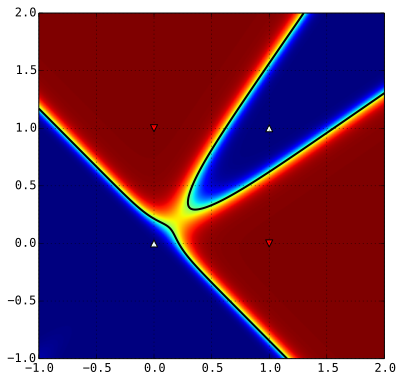
\includegraphics[width=.5\linewidth]{images/mlp.bias0.eps}}
\subfloat[\texttt{Offset + Offset}.\label{fig:mlp.split:bias1}]{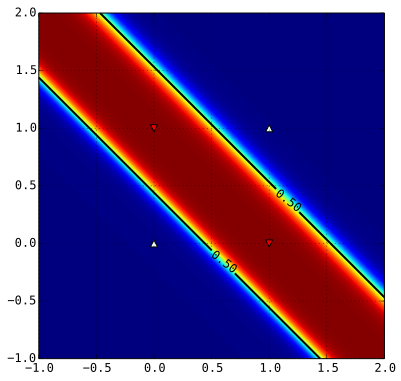
\includegraphics[width=.5\linewidth]{images/mlp.bias1.eps}}
\caption{exclusive OR learned by a three-layer perceptron.\label{fig:mlp.split}}
\end{figure}

同じ境界線でも、加重の初期値を変えて何度も試行すれば、収束に要する時間が変化する様子を観察できる。
余談だが、\subfigref{slp}{judge}に示した論理和の境界線を再現するには、線型分類器を下記の通りに構築し学習する。

\begin{Verbatim}{Scala}
val model = new Offset(2, new Sigmoid, new Output, ()=>new PlainSGD)
for(n<-1 to 1000000; x<-0 to 1; y<-0 to 1) model(Seq(x,y), Seq(x|y))
\end{Verbatim}

\section{鞍点と学習率\label{sect:nn.sgd}}

\eqref{sgd.saddle}に与える関数$E$に対し、原点$\bm{O}$は勾配が$\nabla E\!=\!\bm{0}$であるが、極小点ではない。これを\textbf{鞍点}と呼ぶ。
%
\begin{equation}
\label{eq:sgd.saddle}
\Delta E = \pdiff{f}{x} \Delta x + \pdiff{f}{y} \Delta y = 2x \Delta x - 2y \Delta y\;\where E(x,y) = x^2 - y^2.
\end{equation}

\subfigref{sgd}{avoid}に示す通り、鞍点の近傍では\eqref{mlp.sgd}の勾配法は停滞し、運悪く鞍点に嵌れば、そこで収束する。
\subfigref{sgd}{speed}は、5個の初期値で排他的論理和を学習した際の誤差$\Esq$の推移だが、学習の停滞が観察できる。

\begin{figure}[h]
\centering
\subfloat[saddle point avoidance mechanism.\label{fig:sgd:avoid}]{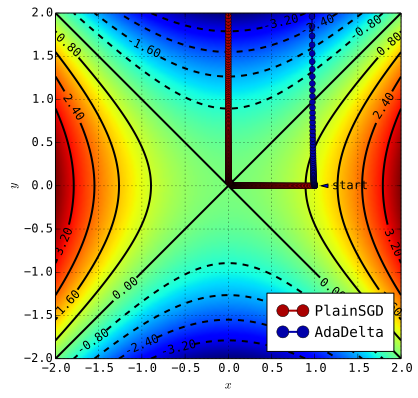
\includegraphics[width=.5\linewidth]{images/sgd.avoid.eps}}
\subfloat[loss diminution through training.\label{fig:sgd:speed}]{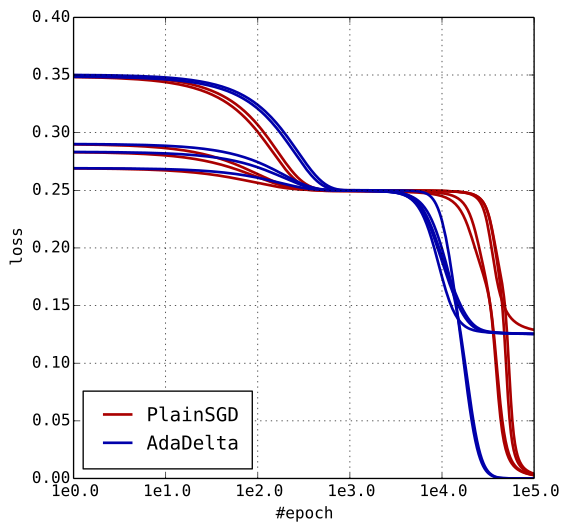
\includegraphics[width=.5\linewidth]{images/sgd.speed.eps}}
\caption{comparison of \texttt{PlainSGD} and \texttt{AdaDelta}.\label{fig:sgd}}
\end{figure}

対策として、最適解の近傍で学習率を小さく、鞍点の近傍では大きく設定する\textbf{適応的勾配法}が効果的である。
\eqref{sgd.adagrad}に示す\textit{AdaGrad}は、学習率を勾配$\nabla E_{mt}^{ij}$の期待値に反比例させつつ、時刻$t$に伴って減衰させる。
%
\begin{equation}
\label{eq:sgd.adagrad}
\Delta w_{mt}^{ij} = -\frac{\eta}{t\sqrt{\E{(\nabla E_m^{ij})^2}_t}}\;
\where \E{(\nabla E_m^{ij})^2}_t = \frac{1}{t} \sum_{\tau=0}^t (\nabla E_{mt}^{ij})^2,\;
\E{(\nabla E_m^{ij})^2}_0 = \varepsilon.
\end{equation}

\eqref{sgd.adadelta}に示す\textit{AdaDelta}は、直近の勾配を重視する。加重$w_m^{ij}$と勾配$\nabla E_m^{ij}$の\textbf{スケール変換}の効果も持つ。
%
\begin{equation}
\label{eq:sgd.adadelta}
\Delta w_{mt}^{ij} = -\frac{\sqrt{\E{(\Delta w_m^{ij})^2}_t+\varepsilon}}{\sqrt{\E{(\nabla E_m^{ij})^2}_t+\varepsilon}} \nabla E_{mt}^{ij}\;
\where \E{x}_t = \rho \E{x}_{t-1} + (1-\rho) x_t,\;
\E{x}_0 = 0.
\end{equation}

下記の\texttt{AdaDelta}クラスに実装する。引数\texttt{r}は係数$\rho$を表す。また、引数\texttt{e}は\textbf{ゼロ除算}を防ぐ係数$\varepsilon$である。

\begin{Verbatim}{Scala}
class AdaDelta(r: Double = 0.95, e: Double = 1e-8) extends SGD {
	var eW,eE = 0.0
	def update(E: Double) = {
		this.eE = r*eE + (1-r) * math.pow(1*E, 2)
		val n = math.sqrt(eW+e) / math.sqrt(eE+e)
		this.eW = r*eW + (1-r) * math.pow(n*E, 2)
		this.w -= n * E
	}
}
\end{Verbatim}

\texttt{PlainSGD}クラスで\subfigref{sgd}{avoid}の軌跡を描くには419回の更新を要したが、\texttt{AdaDelta}クラスは66回である。

\section{多クラス分類\label{sect:nn.mcp}}

出力$y\!\in\!\seq{1,...,K}$の分類器の活性化関数は、関数$\sigm$を$K$クラスに拡張した\textbf{ソフトマックス関数}を使う。
%
\begin{equation}
\label{eq:mcc.smax}
y \sim q(y) = \smax(\bm{z}) = \frac{f_\mathrm{exp}(\bm{z})}{\|f_\mathrm{exp}(\bm{z})\|}\;
\where f_\mathrm{exp}(\bm{z}) = \trans{\begin{pmatrix}e^{z_1} \cdots e^{z_K}\end{pmatrix}}.
\end{equation}

直感的には、最適な事後分布$q(y)$は正解$p(t)$との差を表す\nKL 情報量$\KL{p}{q}$を最小化する。
\nKL 情報量は非負で、\eqref{mcc.KL}に示す\textbf{ギブスの不等式}より$q\!=\!p$に限り$\KL{p}{q}\!=\!0$が成立する。
%
\begin{equation}
\label{eq:mcc.KL}
\KL{p}{q} = \int_K p(y) \log \frac{p(y)}{q(y)} dy \geq \int_K p(y) \left(1-\frac{q(y)}{p(y)}\right) dy = 0\;\leftarrow \log x \leq x-1.
\end{equation}

通常は$\KL{p}{q}$の上限を与える\eqref{mlp.E.ce}の交差エントロピー$\Ece$を通じて、間接的に$\KL{p}{q}$を最小化する。
理由は、出力層の直前の勾配$\nabla{}\Ece(\bm{z})$が\eqref{mcc.gE.ce}で容易に求まり、\eqref{mlp.E.ce}で$H(p)$が定数である点にある。
%
\begin{equation}
\label{eq:mcc.gE.ce}
\pdiff{\Ece}{z_k}
= - \pdiff{}{z_k} \sum_{i=1}^K t_i \left(\log e^{z_i} - \log \sum_{j=1}^K e^{z_j}\right)
= - t_k + \sum_{i=1}^K t_i y_k = -t_k + y_k.
\end{equation}

下記の\texttt{Softmax}クラスに\eqref{mcc.smax}を実装する。出力層の直前での利用を前提に、逆伝播は恒等関数にした。

\begin{Verbatim}{Scala}
class Softmax extends Active {
	def fp(z: Seq[Double]) = z.map(math.exp(_)/z.map(math.exp).sum)
	def bp(z: Seq[Double]) = z.map(_=>1.0)
}
\end{Verbatim}

\texttt{Softmax}クラスは、出力層の直前での利用に限定される点を除き、他の活性化関数と同じ要領で利用できる。

\begin{Verbatim}{Scala}
val model3 = new Output(4, _-_)
val model2 = new Offset(3, new Softmax, model3, ()=>new PlainSGD)
val model1 = new Offset(2, new Sigmoid, model2, ()=>new PlainSGD)
\end{Verbatim}

\figref{mcp.zflag}は、$xy$軸上の4点を標本に与えて、3層パーセプトロンで国際信号旗の\textit{zulu}を学習した結果である。

\begin{figure}[h]
\centering
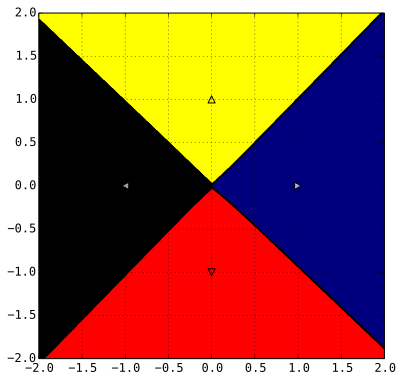
\includegraphics[width=.5\linewidth]{images/mcp.zflag.eps}
\caption{maritime signal flag \textit{zulu} learned by a three-layer perceptron.\label{fig:mcp.zflag}}
\end{figure}

原理上は、\sectref{nn.mlp}と同様に2乗誤差$\Esq$で学習できるが、勾配$\nabla{}\Esq$が緩慢なため、収束に時間がかかる。

\chapter{サポートベクターマシン\label{chap:svm}}

\textbf{サポートベクターマシン}とは、\figref{svm}に示す\textbf{判別境界}を学習し、標本$\seq{\bm{x}_i}$を正負に分割する分類器である。
両側の集団からの最短距離$d$が最大になる直線を学習することで、未知の$\bm{x}$を誤分類する可能性を抑制する。

\begin{figure}[h]
\centering
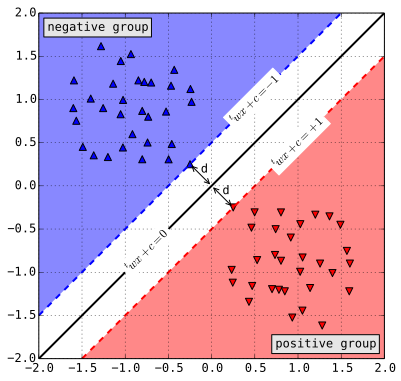
\includegraphics[width=.5\linewidth]{images/svm.model.eps}
\caption{a support vector machine.\label{fig:svm}}
\end{figure}

判別境界$\dprod{\bm{w}\!}{\!\bm{x}}\!+\!c\!=\!0$の学習は\textbf{制約付き最大化問題}であり、標本$\seq{\bm{x}_i,t_i}$は条件\eqref{svm.hard}を満たす必要がある。
%
\begin{equation}
\label{eq:svm.hard}
t_i(\dprod{\bm{w}}{\bm{x}_i} + c) \geq 1\;
\where t_i=
\begin{cases}
+1 & \text{if $\bm{x}_i\in\mathrm{positive\;group}$} \\
-1 & \text{if $\bm{x}_i\in\mathrm{negative\;group}$}
\end{cases}
\end{equation}

ただし、$t_i$は点$\bm{x}_i$が帰属する集団を示す変数である。集団と判別境界との距離$d$は、\eqref{svm.d}で計算できる。
%
\begin{equation}
\label{eq:svm.d}
d(\seq{\bm{x}_i}) = \min\frac{|\dprod{\bm{w}}{\bm{x}_i} + c|}{\|\bm{w}\|} = \frac{1}{\|\bm{w}\|}.
\end{equation}

現実には、正負の境界が曖昧な場合には、\eqref{svm.hard}の遵守が困難なため、\textbf{ソフトマージン}による緩和を図る。
即ち、制約条件を\eqref{svm.soft}に変更し、若干の誤分類を見逃す代わりに、誤分類点$\bm{x}_i$にヒンジ損失$\xi_i$を課す。
%
\begin{equation}
\label{eq:svm.soft}
t_i (\dprod{\bm{w}}{\bm{x}_i} + c) \geq 1 - \xi_i\;
\where \xi_i =
\begin{cases}
0 & \text{if $t_i(\dprod{\bm{w}}{\bm{x}_i} + c) > 1$} \\
|t_i - (\dprod{\bm{w}}{\bm{x}_i} + c)| & \text{if $t_i(\dprod{\bm{w}}{\bm{x}_i} + c) \leq 1$}.
\end{cases}
\end{equation}

誤分類の抑制と距離$d$の最大化は、\eqref{svm.main}の最小化で達成する。ここで、$\|\bm{w}\|^2$はL2正則化の役割を担う。
%
\begin{equation}
\label{eq:svm.main}
f(\seq{\bm{x}_i,t_i}, \bm{w}, c) = C \sum_{i=1}^N \xi_i + \frac{1}{2}\|\bm{w}\|^2 \where C>0.
\end{equation}

誤分類点の集合$E(\seq{\bm{x}_i})$に対し、\eqref{svm.C}が成立する。故に、定数$C$は誤分類率の限度を間接的に決定する。
%
\begin{equation}
\label{eq:svm.C}
\sum_{i=1}^N \xi_i > |E(\seq{\bm{x}_i})|
\leftarrow
\forall \bm{x}_i \in E(\seq{\bm{x}_i}),\;\xi_i>1.
\end{equation}

\section{凸二次計画問題\label{sect:svm.smo}}

\eqref{svm.main}の最小化は、未定乗数法と\KKT 条件の適用により、\textbf{凸二次計画問題}で達成できる。
%
\begin{equation}
\label{eq:svm.L}
L(\bm{w},c,\xi,\lambda,\mu)
= \frac{1}{2}\|\bm{w}\|^2 +C \sum_{i=1}^N \xi_i - \sum_{i=1}^N \lambda_i \{t_i(\dprod{\bm{w}}{\bm{x}_i} + c) - 1\} - \sum_{i=1}^N \mu_i \xi_i.
\end{equation}

$\lambda_i$と$\mu_i$は座標$\bm{x}_i$に関する未定乗数である。係数$\bm{w}$と$c$で偏微分して、$L$が最小になる条件\eqref{svm.dual}を得る。
%
\begin{equation}
\label{eq:svm.dual}
\tilde{L}(\lambda)
= \min_{\bm{w},c} L(\bm{w},c, \lambda)
= \sum_{i=1}^N \lambda_i \seq{1 - \frac{1}{2} \sum_{j=1}^N \lambda_j t_i t_j (\dprod{\bm{x}_i}{\bm{x}_j})}
\where\left\{
\begin{aligned}
0         &= \sum_{i=1}^N \lambda_i t_i \\
\lambda_i &= C - \mu_i\\
\bm{w}    &= \sum_{i=1}^N \lambda_i t_i \bm{x}_i
\end{aligned}
\right..
\end{equation}

\eqref{svm.soft}は不等式ゆえ、\KKT 条件より、\eqref{svm.dual}が最適解を与える場合、\eqref{svm.kkt}を満たす。
誤分類点の存在を無視すると、\eqref{svm.dual}\eqref{svm.kkt}より、判別境界から距離$d$の点のみが係数$\bm{w}$の決定に寄与する。
%
\begin{equation}
\label{eq:svm.kkt}
\lambda_i \seq{t_i\left(\sum_{j=1}^N \lambda_j t_j \dprod{\bm{x}_j}{\bm{x}_i} + c\right) + \xi_i - 1} = 0\;
\where\left\{
\begin{aligned}
\lambda_i &\geq 0 \\
\mu_i     &\geq 0 \\
\mu_i\xi_i&=0
\end{aligned}
\right..
\end{equation}

これを\textbf{サポートベクトル}と呼ぶ。より遠方の点は、$\lambda_i\!=\!0$を満たす必要から、係数$\bm{w}$の決定に無関係である。
以後、双対問題$\tilde{L}(\lambda)$を最大化する。今回は、実装が容易で計算が高速な\textbf{逐次最小問題最適化法}を利用する。
%
\begin{equation}
\label{eq:svm.smo.d}
t_i \delta_i + t_j \delta_j = 0\;
\where \left\{
\begin{aligned}
\delta_i &= \hat{\lambda}_i - \lambda_i \\
\delta_j &= \hat{\lambda}_j - \lambda_j
\end{aligned}
\right\}\;
\leftarrow 0 = \sum_{i=1}^N \lambda_i t_i.
\end{equation}

これは、\eqref{svm.kkt}を破る点$\bm{x}_i$が存在する限り、任意の点$\bm{x}_j$を選び、\eqref{svm.smo.d}を満たす局所的な最適化を施す。
\eqref{svm.dual}の$\tilde{L}(\lambda)$から、1回の最適化による$\lambda_i,\lambda_j$の増分$\delta_i$,$\delta_j$を含む部分式を抜き出すと、\eqref{svm.smo.dL}を得る。
%
\begin{equation}
\label{eq:svm.smo.dL}
d\tilde{L}(\delta_i, \delta_j) =
\delta_i +\delta_j -
\frac{1}{2} |\delta_i t_i \bm{x}_i + \delta_j t_j \bm{x}_j|^2 -
\sum_{n=1}^N \lambda_n t_n \dprod{\bm{x}_n}{(\delta_i t_i \bm{x}_i + \delta_j t_j \bm{x}_j)}.
\end{equation}

\eqref{svm.smo.dL}に\eqref{svm.smo.d}の制約を加えると、\eqref{svm.smo.dL.di}を得る。なお、\eqref{svm.smo.dL.di}は変数$t_i$の符号に拘らず成立する。
%
\begin{equation}
\label{eq:svm.smo.dL.di}
d\tilde{L}(\delta_i) =
t_i (t_i - t_j) \delta_i -
\frac{1}{2} \delta_i^2 |\bm{x}_i - \bm{x}_j|^2 -
t_i \delta_i \sum_{n=1}^N \lambda_n t_n \dprod{\bm{x}_n}{(\bm{x}_i - \bm{x}_j)}.
\end{equation}

双対問題$\tilde{L}(\lambda)$の最大化は、$d\tilde{L}(\delta_i,\delta_j)$の極大点の探索と同義である。$\delta_i$での偏微分により、\eqref{svm.smo}を得る。
なお、更新後の値$\hat{\lambda}_i$と$\hat{\lambda}_j$が\eqref{svm.kkt}を逸脱する場合は、\textbf{クリッピング}により強制的に区間$[0,C]$に収める。
%
\begin{equation}
\label{eq:svm.smo}
\delta_i = - \frac{t_i}{|\bm{x}_i - \bm{x}_j|^2} \seq{\sum_{n=1}^N \lambda_n t_n \dprod{\bm{x}_n}{(\bm{x}_i - \bm{x}_j)} - t_i + t_j}.
\end{equation}

座標$\bm{x}_i$に対し、条件\eqref{svm.kkt}を確認する際は、係数$\bm{w}$と$c$の値が必要になるが、$\bm{w}$の値は\eqref{svm.dual}で求まる。
定数項$c$の値は、$t_i(\dprod{\bm{w}\!}{\!\bm{x}_i})$を最小化する座標$\bm{x}_i$がサポートベクトルとなる点に着目し、\eqref{svm.smo.c}で求める。
%
\begin{equation}
\label{eq:svm.smo.c}
c = -\frac{1}{2} \seq{
\min_{i|t_i=+1} \sum_{j=1}^N \lambda_j t_j \dprod{\bm{x}_i}{\bm{x}_j} +
\max_{j|t_j=-1} \sum_{i=1}^N \lambda_i t_i \dprod{\bm{x}_j}{\bm{x}_j}}.
\end{equation}

下記の\texttt{SVM}クラスはサポートベクターマシンを実装する。標本$\seq{\bm{x}_i}$は引数\texttt{X}に渡す。引数\texttt{k}は内積を表す。

\begin{Verbatim}{Scala}
class SVM(X: Seq[(Seq[Double],Int)], C: Double, k: (Seq[Double],Seq[Double])=>Double) {
	val data = X.map(Data.tupled)
	var c = 0.0
\end{Verbatim}

\texttt{SVM}クラス内に\texttt{Data}クラスを実装する。これは、標本の$i$番目の点$\bm{x}_i$と正解$t_i$と未定乗数$\lambda_i$を記憶する。

\begin{Verbatim}{Scala}
	case class Data(x: Seq[Double], t: Int) {
		var l = 0.0
	}
\end{Verbatim}

判別境界を表す係数$\bm{w}$は変数に記憶せず、内積$\dprod{\bm{w}\!}{\!\bm{x}}$の形で実装する。これは\sectref{svm.kern}に向けた布石である。

\begin{Verbatim}{Scala}
	def wx(x: Data) = data.map(d => d.l * d.t * k(x.x,d.x)).sum
\end{Verbatim}

\texttt{kkt}メソッドは、\eqref{svm.kkt}の\KKT 条件を検査する。実数の比較では\textbf{丸め誤差}に注意を払う。

\begin{Verbatim}{Scala}
	def kkt(x: Data) = (x.t * this(x.x) - 1) match {
		case e if e < -1e-10 => x.l >= C
		case e if e > +1e-10 => x.l <= 0
		case _ => true
	}
\end{Verbatim}

\texttt{clip}メソッドは、\eqref{svm.smo}の最適化を行う際に、未定定数の差分$\delta_i$と$\delta_j$の閉区間$[0,C]$からの逸脱を防ぐ。

\begin{Verbatim}{Scala}
	def clip(xi: Data, xj: Data, d: Double): Double = {
		if(d < lower(xi, xj)) return lower(xi, xj)
		if(d > upper(xi, xj)) return upper(xi, xj)
		return if(d.isNaN) 0 else d
	}
\end{Verbatim}

\texttt{lower}メソッドは、差分$\delta_i$や$\delta_j$の下限を計算する。下限は\eqref{svm.smo.d}の$\delta_i$の定義と\eqref{svm.dual}\eqref{svm.kkt}から導ける。

\begin{Verbatim}{Scala}
	def lower(xi: Data, xj: Data) = xi.t * xj.t match {
		case  1 => math.max(-xi.l, +xj.l - C)
		case -1 => math.max(-xi.l, -xj.l)
	}
\end{Verbatim}

同様に、差分$\delta_i$や$\delta_j$の上限も\eqref{svm.smo.d}の$\delta_i$の定義と\eqref{svm.dual}\eqref{svm.kkt}から導出し、\texttt{upper}メソッドに実装する。

\begin{Verbatim}{Scala}
	def upper(xi: Data, xj: Data) = xi.t * xj.t match {
		case  1 => math.min(+xj.l, -xi.l + C)
		case -1 => math.min(-xi.l, -xj.l) + C
	}
\end{Verbatim}

次に実装する\texttt{pos}と\texttt{neg}は、正負のサポートベクトルの内積$\dprod{\bm{w}\!}{\!\bm{x}}$を求める。\eqref{svm.smo.c}を計算する際に使う。

\begin{Verbatim}{Scala}
	def pos = data.filter(_.t == +1).map(wx(_)).min
	def neg = data.filter(_.t == -1).map(wx(_)).max
\end{Verbatim}

下記は、逐次最小問題最適化法の反復処理である。\eqref{svm.kkt}を破る点$\bm{x}_i$を探し、\eqref{svm.smo}に従って更新する。

\begin{Verbatim}{Scala}
	while(data.count(!kkt(_)) >= 2) {
		val a = data.find(!kkt(_)).get
		val b = data(util.Random.nextInt(X.size))
		val sub = wx(Data((a.x,b.x).zipped.map(_-_), 0))
		val den = k(a.x,a.x) - 2*k(a.x,b.x) + k(b.x,b.x)
		val del = clip(a, b, -a.t * (sub-a.t+b.t) / den)
		a.l += del
		b.l -= del * a.t * b.t
		this.c = -0.5 * (pos+neg)
	}
\end{Verbatim}

下記の\texttt{apply}メソッドは、未知の点$\bm{x}$に対して$\dprod{\bm{w}\!}{\!\bm{x}}\!+\!c$を計算する。返り値の正負は、帰属する集団を表す。

\begin{Verbatim}{Scala}
	def apply(x: Seq[Double]) = wx(Data(x, 0)) + c
}
\end{Verbatim}

完成した\texttt{SVM}クラスを使う際は、標本$\bm{x}_i$に加え、ソフトマージンの定数$C$と内積の定義を引数に指定する。

\begin{Verbatim}{Scala}
val svm = new SVM(data, 1e-10, (a, b) => (a, b).zipped.map(_*_).sum)
\end{Verbatim}

\figref{svm.line}は、線型分離可能な標本を\texttt{SVM}クラスで学習した結果である。ただし\subref{fig:svm.line:2}は2個の誤分類点を含む。
黒の点線は判別境界を表し、赤と青の点線は$\dprod{\bm{w}\!}{\!\bm{x}}\!+\!c\!=\!\pm1$を表す。赤と青の濃淡は$\dprod{\bm{w}\!}{\!\bm{x}}\!+\!c$の相対値を表す。

\begin{figure}[h]
\centering
\subfloat[sample data separable by a line.\label{fig:svm.line:1}]{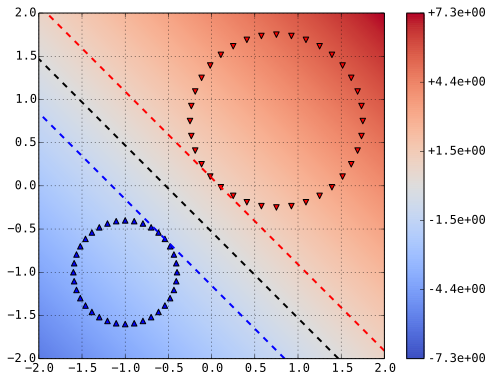
\includegraphics[width=.5\linewidth]{images/svm.line1.eps}}
\subfloat[sample data with outlier points.\label{fig:svm.line:2}]{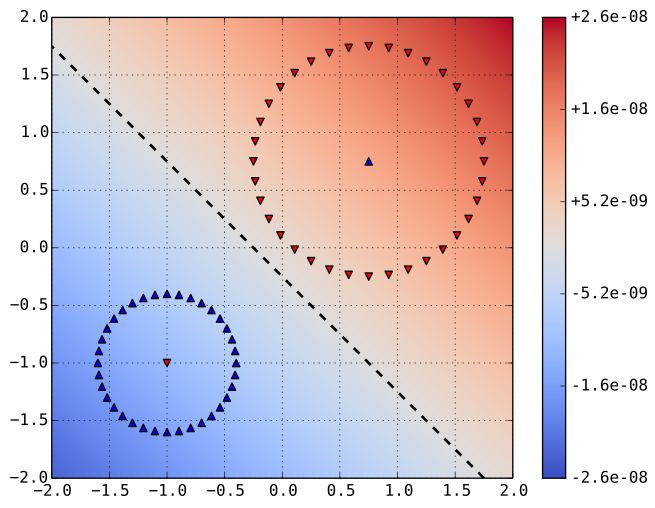
\includegraphics[width=.5\linewidth]{images/svm.line2.eps}}
\caption{decision surface learned by a linear SVM.\label{fig:svm.line}}
\end{figure}

\subref{fig:svm.line:1}は、両集団を直線で完璧に分離できる場合、判別境界がサポートベクトルの中間に位置する様子を表す。
\subref{fig:svm.line:2}は、判別境界が正の領域にある負の誤分類点に誘引され、かつサポートベクトルが消滅する様子を表す。

\section{特徴空間の変換\label{sect:svm.kern}}

\sectref{svm.kern}では、サポートベクターマシン等の\textbf{線型分類器}を非線型分離な問題に対応させる\textbf{カーネル法}を学ぶ。
根底には、標本を高次元空間に写像することで、像の分布を疎にした上で、線型分離を達成する着想がある。
%
\begin{equation}
\label{eq:kern.map}
\Phi: \bm{x} \mapsto \Phiz\;\;
\mathrm{e.g.}\;
\begin{pmatrix}x\\y\end{pmatrix} \mapsto z=\frac{1}{2\pi} \exp \left(-\frac{x^2 + y^2}{2}\right).
\end{equation}

\figref{svm.trick}は、同心円に並ぶ正負の集団を\eqref{kern.map}で$z$軸上に投影し、$z$軸に垂直な分離平面を得る例である。

\begin{figure}[h]
\centering
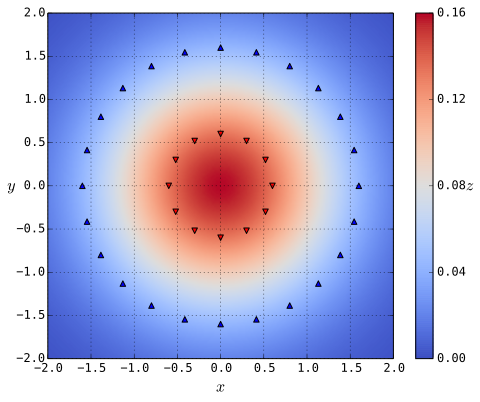
\includegraphics[width=.5\linewidth]{images/svm.trick.eps}
\caption{conversion of linearly inseparable problem to separable.\label{fig:svm.trick}}
\end{figure}

\eqref{svm.hard}--\ref{eq:svm.smo.c}の座標$\bm{x}$を$\Phiz$に変更し、\sectref{svm.kern}の議論に流用する。例えば、係数$\bm{w}$は\eqref{kern.w}で求める。
基本的に、像$\Phiz$の次元$D$が高ければ分離の機会は増えるが、\eqref{svm.hard}--\ref{eq:svm.smo.c}の計算は$\mathcal{O}(D)$の時間を要する。
%
\begin{equation}
\label{eq:kern.w}
\bm{w} = \sum_{i=1}^N \lambda_i t_i \Phix{i}.
\end{equation}

ここで、\eqref{svm.kkt}\eqref{svm.smo}\eqref{svm.smo.c}を注意深く観察すると、内積$\dprod{\Phix{i}\!}{\!\Phix{j}}$が求まれば$\Phiz$の値は不要な点に気付く。
実は、像の計算を経ず内積を計算する手段が存在する。まず、\eqref{kern.k}に示す2変数の\textbf{対称関数}を定義する。
%
\begin{equation}
\label{eq:kern.k}
k: \mathbb{M} \times \mathbb{M} \to \mathbb{R}\;\where k(\bm{x}_i,\bm{x}_j) = k(\bm{x}_j,\bm{x}_i).
\end{equation}

記号$\mathbb{M}$は\textbf{可測空間}を指す。関数$k$は、\eqref{kern.pos}に示す\textbf{正定値性}を満たす場合、\textbf{正定値カーネル}と呼ばれる。
%
\begin{equation}
\label{eq:kern.pos}
\forall \bm{x}\in\mathbb{R}^n,\;
\trans{\bm{x}}
\begin{pmatrix}
k(\bm{x}_1,\bm{x}_1) & \cdots & k(\bm{x}_1,\bm{x}_n) \\
\vdots & \ddots & \vdots \\
k(\bm{x}_n,\bm{x}_1) & \cdots & k(\bm{x}_n,\bm{x}_n) \\
\end{pmatrix}
\bm{x} > 0.
\end{equation}

\eqref{kern.pos}の関数$k$に対し、\eqref{kern.H}の像$\Phix{i}$の線型結合からなる空間$H_k$を\textbf{再生核ヒルベルト空間}と呼ぶ。
%
\begin{equation}
\label{eq:kern.H}
H_k = \seq{f(\bm{x}) = \sum_{n=1}^N a_n \Phix{n} = \sum_{n=1}^N a_n k(\bm{x}, \bm{x}_n)}
\where \Phi: \bm{x} \mapsto \Phix{n} = k(\bm{x}, \bm{x}_n).
\end{equation}

空間$H_k$の元$f$と$g$に対し、内積$\iprod{f}{g}$は非退化かつ正定値な\textbf{対称双線型形式}であり、\eqref{kern.iprod}で定義する。
%
\begin{equation}
\label{eq:kern.iprod}
\iprod{f}{g} = \sum_{i=1}^N \sum_{j=1}^N a_i b_j k(\bm{x}_i, \bm{x}_j)\;
\where\left\{
\begin{aligned}
f(\bm{x}) &= \sum_{i=1}^N a_i k(\bm{x}, \bm{x}_i) \\
g(\bm{x}) &= \sum_{j=1}^N b_j k(\bm{x}, \bm{x}_j) \\
\end{aligned}
\right\}\;
a_i,b_j \in \mathbb{R}.
\end{equation}

余談ながら、内積と距離を備え、かつ\textbf{完備}な空間を\textbf{ヒルベルト空間}と呼び、\eqref{kern.rep}の性質を\textbf{再生性}と呼ぶ。
%
\begin{equation}
\label{eq:kern.rep}
\iprod{f}{k(\bm{x},\bm{x}_j)} = \sum_{i=1}^N a_i k(\bm{x}_i, \bm{x}_j) = f(\bm{x}_j).
\end{equation}

\eqref{kern.rep}の性質は、像$\Phix{i}$や$\Phix{j}$の明示的な計算を経ずに、内積$\dprod{\Phix{i}\!}{\!\Phix{j}}$の値が求まる可能性を示唆する。
この技法は\textbf{カーネルトリック}と通称される。関数$k$の定義次第では、無限次元の空間への変換も可能である。
%
\begin{equation}
\label{eq:kern.example}
\dprod{\Phix{i}}{\Phix{j}} = k(\bm{x}_i,\bm{x}_j) = \left\{
\begin{aligned}
& \sum_{d=1}^D x_{id} x_{jd} && \text{$\cdots$ linear kernel} \\
& \exp \left(-\frac{|\bm{x}_i - \bm{x}_j|^2}{2\sigma^2}\right) && \text{$\cdots$ Gaussian kernel}
\end{aligned}
\right.
\end{equation}

\eqref{kern.example}のうち\textbf{線型カーネル}は単なる恒等変換に過ぎないが、\textbf{ガウシアンカーネル}には興味深い特性がある。
%
\begin{equation}
\label{eq:kern.gauss}
\exp \frac{\dprod{\bm{x}_i}{\bm{x}_j}}{\sigma^2}
= \exp \sum_{d=1}^D \frac{x_{id} x_{jd}}{\sigma^2}
= \prod_{d=1}^D \exp \frac{x_{id} x_{jd}}{\sigma^2}
= \prod_{d=1}^D \sum_{n=0}^\infty
\frac{1}{\sqrt{n!}} \left(\frac{x_{id}}{\sigma}\right)^n
\frac{1}{\sqrt{n!}} \left(\frac{x_{jd}}{\sigma}\right)^n.
\end{equation}

\eqref{kern.gauss}は、\eqref{kern.gauss.base}のような無限次元のベクトルの内積と同義であり、事実上、無限次元への写像を表す。
%
\begin{equation}
\label{eq:kern.gauss.base}
\sum_{n=0}^\infty
\frac{1}{\sqrt{n!}} \left(\frac{x_{id}}{\sigma}\right)^n
\frac{1}{\sqrt{n!}} \left(\frac{x_{jd}}{\sigma}\right)^n =
\begin{pmatrix}
\frac{1}{\sqrt{0!}} \left(\frac{x_{id}}{\sigma}\right)^0 \\
\vdots \\
\frac{1}{\sqrt{n!}} \left(\frac{x_{id}}{\sigma}\right)^n \\
\vdots
\end{pmatrix}
\cdot
\begin{pmatrix}
\frac{1}{\sqrt{0!}} \left(\frac{x_{jd}}{\sigma}\right)^0 \\
\vdots \\
\frac{1}{\sqrt{n!}} \left(\frac{x_{jd}}{\sigma}\right)^n \\
\vdots
\end{pmatrix}
\end{equation}

他の著名なカーネルの例では、\eqref{kern.tanh}の\textbf{シグモイドカーネル}は3層パーセプトロンに似た挙動で知られる。
%
\begin{equation}
\label{eq:kern.tanh}
\mathrm{sign}\left(\dprod{\bm{w}}{\Phiz} + c\right) = \mathrm{sign}\left(\sum_{i=1}^N \lambda_it_i k_s(\bm{x},\bm{x}_i) + c\right)\;
\where k(\bm{x}_i, \bm{x}_j) = \tanh \left(c \sum_{d=1}^D x_{id} x_{jd} + \theta\right).
\end{equation}

\figref{svm.kern}は、\texttt{SVM}クラスの引数$\texttt{k}$にガウシアンカーネルを与えて、非線型分離な標本を学習した結果である。

\begin{figure}[h]
\centering
\subfloat[diamond-shaped samples.]{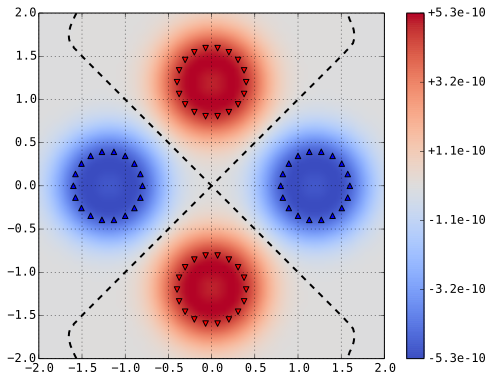
\includegraphics[width=.5\linewidth]{images/svm.kern1.eps}}
\subfloat[two concentric circles.]{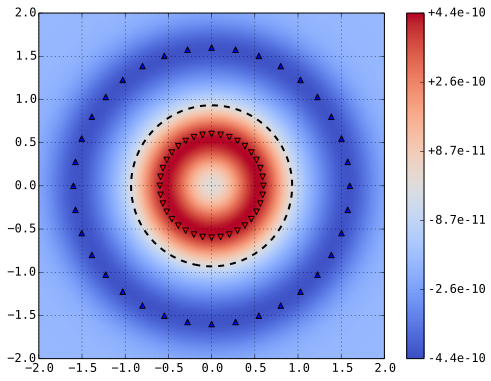
\includegraphics[width=.5\linewidth]{images/svm.kern2.eps}}
\caption{decision surface learned by a Gaussian SVM.\label{fig:svm.kern}}
\end{figure}

黒の点線は判別境界を表し、赤と青の濃淡は$\dprod{\bm{w}\!}{\!\bm{x}}\!+\!c$の相対値を表す。カーネル法の利点がよく理解できる。

\end{document}
